\documentclass{book}

\usepackage[utf8]{inputenc}
\usepackage[spanish]{babel}

% Graphics
\usepackage[left=3cm,right=2cm,top=2cm,bottom=2cm]{geometry} 
\usepackage{graphicx}
\usepackage{xcolor} 
\graphicspath{ {./images/} }

% Math
\usepackage{amssymb}
\usepackage{amsmath}

% Figures and tables
\usepackage{array}
\usepackage{multirow}

% Enumerations
\usepackage{enumitem}

% Bibliography
\usepackage{csquotes}
\usepackage[backend=biber,style=apa]{biblatex}
\addbibresource{referencias.bib}

% Hyperlinks
\usepackage{hyperref}

% Algorithms
\usepackage[spanish,ruled,vlined]{algorithm2e}

% Code highlighting
\usepackage{listings}

% hyperref setup
\hypersetup{
  colorlinks   = true, %Colours links instead of ugly boxes
  urlcolor     = blue, %Colour for external hyperlinks
  linkcolor    = black, %Colour of internal links
  citecolor   = red %Colour of citations
}

\makeatletter

\colorlet{punct}{red!60!black}
\definecolor{background}{HTML}{EEEEEE}
\definecolor{delim}{RGB}{20,105,176}
\colorlet{numb}{magenta!60!black}
\lstdefinelanguage{json}{
    basicstyle=\normalfont\ttfamily,
    numbers=left,
    numberstyle=\scriptsize,
    stepnumber=1,
    numbersep=8pt,
    showstringspaces=false,
    breaklines=true,
    frame=lines,
    backgroundcolor=\color{background},
    literate=
     *{0}{{{\color{numb}0}}}{1}
      {1}{{{\color{numb}1}}}{1}
      {2}{{{\color{numb}2}}}{1}
      {3}{{{\color{numb}3}}}{1}
      {4}{{{\color{numb}4}}}{1}
      {5}{{{\color{numb}5}}}{1}
      {6}{{{\color{numb}6}}}{1}
      {7}{{{\color{numb}7}}}{1}
      {8}{{{\color{numb}8}}}{1}
      {9}{{{\color{numb}9}}}{1}
      {:}{{{\color{punct}{:}}}}{1}
      {,}{{{\color{punct}{,}}}}{1}
      {\{}{{{\color{delim}{\{}}}}{1}
      {\}}{{{\color{delim}{\}}}}}{1}
      {[}{{{\color{delim}{[}}}}{1}
      {]}{{{\color{delim}{]}}}}{1},
}

% Commands
\newcommand\ProcessThreeDashes{\llap{\color{cyan}\mdseries-{-}-}}
\newcommand{\HRule}{\rule{\linewidth}{0.5mm}} %Lineas


% Highlighting
\definecolor{codegreen}{rgb}{0,0.6,0}
\definecolor{codegray}{rgb}{0.5,0.5,0.5}
\definecolor{codepurple}{rgb}{0.58,0,0.82}
\definecolor{backcolour}{rgb}{0.95,0.95,0.92}
\lstdefinestyle{mystyle}{
    backgroundcolor=\color{backcolour},   
    commentstyle=\color{codegreen},
    keywordstyle=\color{magenta},
    numberstyle=\tiny\color{codegray},
    stringstyle=\color{codepurple},
    basicstyle=\ttfamily\footnotesize,
    breakatwhitespace=false,         
    breaklines=true,                 
    captionpos=b,                    
    keepspaces=true,                 
    numbers=left,                    
    numbersep=5pt,                  
    showspaces=false,                
    showstringspaces=false,
    showtabs=false,                  
    tabsize=2
}

\lstset{style=mystyle}

\title{Chatbot para orientación para la comunidad de ESCOM en el marco normativo}


\author{Allan Garcia}
\date{Enero 2021}

\begin{document}

%
% Title page
%
\begin{titlepage}
		%Header
		\centering
		\begin{figure}
			\begin{minipage}[t]{0.4\textwidth}
    			
\includegraphics[height=80pt]{images/escom}
  			\end{minipage}
  			\hfill
			\begin{minipage}[t]{0.4\textwidth}
				\begin{flushright}
	    			
\includegraphics[height=80pt]{images/ipn}				
				\end{flushright}
  			\end{minipage}
		\end{figure}
		
		
		\textsc{\LARGE Escuela Superior de Cómputo}\\[.2cm]
		\textsc{\LARGE Instituto Politécnico Nacional}\\[1.4cm]
		
		\textsc{\Large Trabajo Terminal \#2019-B040}
		
		Enero    del 2021
		
		%Titulo
		\HRule \\[0.9cm]
			{ \LARGE \bfseries Chatbot para orientación para la comunidad de ESCOM en el marco normativo}\\[0.7cm]
		\HRule \\[1cm]
		
		%Nombres
		\textbf{\Large \emph{Presenta:}}\\[.2cm]
		
		{\large Allan de Jesús García \'{A}lvarez}\\[.8cm]
		
		\textbf{\Large \emph{Director:}}\\[.2cm]
		
		{\large Catalán Salgado Edgar Armando}\\[.8cm]
		
		\textbf{\large Palabras Clave}: procesamiento de lenguaje natural, minería de texto, sistemas de recuperación de información, similitud de semántica.
\end{titlepage}

\tableofcontents

% Estructura general
% Introduccion, estado del arte, marco teorico, analisis, diseño, desarrollo, pruebas, conclusiones, bibliografia, apendices

\chapter{Introducción}


\section{Normatividad escolar y su importancia}

Como seres sociales, existe la necesidad de establecer acuerdos que regulen el comportamiento y las formas de crear relaciones con otros individuos. Estos acuerdos son de suma importancia para facilitar interacciones y las actividades de organizaciones sociales. En algunas ocasiones estos acuerdos mutuos entre individuos llegan a cuestionarse por causas de conflictos de principios. Un estudio ha delimitado tres dominios sobre los cuáles los valores se construyen \parencite{thornberg}:

\begin{itemize}
    \item \textbf{moral}: conceptos de bienestar humano, justicia y verdad.
    \item \textbf{convencional}: conceptos éticos basados en autoridad, tradiciones, consensos y acuerdos.
    \item \textbf{personal}: conceptos que pertenecen principalmente al comportamiento de uno mismo basado en preferencias y decisiones que buscan la mayor satisfacción posible.
\end{itemize}

Esto nos lleva a buscar una referencia en común que se vuelve necesaria para un orden, ya que si no se establecen conceptos uniformes la forma de evaluar el comportamiento se vuelve ambiguo. Se debe tener en alta estima o el respeto hacia un autoridad en común cuando se tratan de valores convencionales. Estas convenciones deben ser vistas como parte de un sistema fijo y requieren adherencia mutua entre individuos \parencite{turiel}.

Mientras que los dominios morales y personales quedan abstraídos en la subjetividad, el dominio convencional se establece bajo la autoridad y uniformidad de comportamiento mediante un \textit{convenios sociales} o \textit{contrato social} que optimiza la integración de todos los individuos de la mejor manera posible. Esto es posible mediante normas que se fundamentan de manera oficial como resultado de este acuerdo con el uso de autoridad. Mediante un sistema de este tipo se puede trasladar este objetivo a los distintos grupos que la sociedad forma para cumplir diferentes funciones.

Para poder enunciar de manera oficial estas bases, se necesitan leyes y reglamentos. Una \textbf{ley} es una norma emitida establecida de manera jurídica por un estado a través de sus poder legislativo del Estado, junto con las consecuencias de la infracción de tales leyes \parencite{davidrogers}. Sin embargo, la ley no da especificación a detalle de lo que consiste el cumplimiento, Son los \textbf{reglamentos} determina los procesos y definiciones a detalle para complementar el efecto jurídico de las normas. 

Un \textbf{marco jurídico} es el conjunto de leyes y normas que forman la base legal. En ella se determinan las formas de organización y funciones de una sociedad. El ejercicio de los marcos jurídicos es sumamente importante para garantizar que se cumplan los derechos que le corresponden a un conjunto de individuos para regular la forma en que se relacionan. Dentro de cualquier ámbito, se debe establecer una autoridad que emita y se encargue de hacer cumplir ciertas normas para que el orden se mantenga de manera óptima para todos.

Un \textbf{marco normativo} son las disposiciones legales que regulan asuntos específicos de los procesos para el funcionamiento de esa sociedad. Es decir, las diversas organizaciones establecen un marco normativo para que una autoridad pueda regular las actividades de las diversas materias que le competen. \textit{El marco jurídico da la base legal para que establezcan las reglas específicas para atender a los procesos esenciales de una organización mediante el marco normativo}.

Ambos conceptos se reducen a la definición de los derechos y obligaciones que un individuo tiene como integrante de una organización y las implicaciones que consisten en su participación. Es por ello que como sociedad se divulgue y se haga del conocimiento a la comunidad interesada. Esto se hace a través de establecer leyes y reglamentos en un \textbf{documento legal}. En México, las leyes y reglamentos se organizan de manera estructural, la cual se debe dividir de acuerdo a la extensión de asuntos que trata un mismo reglamento \parencite{lopezruiz}. Estas divisiones estructurales son las siguientes:

\begin{enumerate}
    \item \textbf{Libros}: recopilan leyes muy extensas que se pueden dividir por su complejidad.
    \item \textbf{Títulos}: utilizado en leyes extensas, esta agrupación divide partes claramente diferenciadas.
    \item \textbf{Capítulos}: tiene un contenido unitario que no es fijado solo con base en el número de artículos sino que dependen de la materia que tratan.
    \item \textbf{Secciones}: utilizado cuando la materia es extensa y requiere subdividir a los artículos, pero no es suficiente para ser tratado como capítulo.
    \item \textbf{Artículos}: unidad normativa que regula un tema o precepto que se dicta de forma de un solo enunciado.
    \item \textbf{Párrafos}: unidad parcial de un artículo que divide la redacción.
    \item \textbf{Apartados}: Utilizado de manera poco común, funciona para dividir todo lo referente a la misma materia normativa. Se deben diferenciar con letras mayúsculas.
    \item \textbf{Fracciones}: Enumeran una serie de atribuciones, requisitos, obligaciones, etc, otorgados en un artículo. Se separan con números romanos.
    \item \textbf{Incisos}: División mínima legal utilizada para enumerar elementos o lista de objetos y entidades como componentes de la misma norma. Se numeran con letras minúsculas cerradas por medio de paréntesis de cierre, sin punto ni guión.
\end{enumerate}

Siendo la estructura temática un aspecto esencial de la ley, se debe resaltar que son los \textbf{artículos} la división elemental y fundamental de las leyes que constituye una disposición atómica. Esta misma estructura aplica a asuntos internos de diversas instituciones, que requieren establecer sus normas para que sus integrantes se adhieran en todo momento para cumplir con las finalidades establecidas.


\subsection{Marco Normativo del Instituto Politécnico Nacional}
\label{subsec:marco-normativo-ipn}

El Instituto Politécnico Nacional se rige por su propia Ley Orgánica y se encuentra capaz de expedir los acuerdos en los que se dictan los reglamentos necesarios para el cumplimiento de los objetivos académicos y supervisar que los procesos incluidos en el marco normativo sean apegados a los mismos reglamentos para regular la vida social y el desarrollo profesional de sus integrantes.

El artículo 3 de la Constitución Política de los Estados Unidos Mexicanos dicta que:

\begin{quote}
    \textit{La educación se basará en el respeto irrestricto de la dignidad de las personas, con un enfoque de derechos humanos y de igualdad sustantiva. Tenderá a desarrollar armónicamente todas las facultades del ser humano y fomentará en él, a la vez, el amor a la Patria, el respeto a todos los derechos, las libertades, la cultura de paz y la conciencia de la solidaridad internacional, en la independencia y en la justicia; promoverá la honestidad, los valores y la mejora continua del proceso de enseñanza aprendizaje.}
\end{quote}

Es este principio el que da la base para que las actividades desarrolladas por el Instituto Politécnico tengan un sentido social humano equitativo para todos sus integrantes en beneficio del país. Actualmente existen 29 reglamentos. Estos reglamentos derivan a cada dependencia del instituto, incluyendo a la Escuela Superior de Cómputo (ESCOM). El marco normativo de la ESCOM completamente de las disposiciones emitidas por el Instituto Politécnico Nacional, que a su vez se le considera como un \textit{órgano desconcentrado de la Secretaría de Seguridad Pública, cuya orientación general corresponde al Estado}, de acuerdo con el artículo 2 de la Ley Orgánica del Instituto Politécnico Nacional.


De esta manera, la ESCOM participa en el ejercicio de un sistema de normas que ayudan a establecer procesos y reglamentos que exigen el cumplimiento de obligaciones, pero usando su derecho en todo momento cuando su comunidad académica realiza las actividades cotidianas correspondientes a sus funciones. Como por ejemplo, la forma en cómo se regulan las opciones de titulación quedan establecidas en el \textit{Reglamento de Titulación Profesional}. El marco normativo también da vigencia a las autoridades escolares mediante la \textit{Ley Orgánica}.

\subsection{La importancia de la divulgación}

Todo integrante de esta comunidad de la Escuela Superior de Cómputo queda implicado en la práctica de las normas en todo momento. Por lo tanto, el marco normativo debe ser referencia y se debe hacer de su conocimiento. 

\begin{figure}
    \centering
    
\includegraphics[scale=0.225]{images/1/pagina-normatividad.png}
    \caption{Captura de pantalla del sitio con el contenido referente al marco normativo del IPN.}
    \label{fig:sitio-normatividad}
\end{figure}

Los recursos que conforman parte de este marco normativo se pueden encontrar dentro del sitio \url{https://www.ipn.mx/normatividad/}. La figura \ref{fig:sitio-normatividad} muestra una captura de pantalla de este sitio que contiene categorías distintas para la ubicación de documentos emitidos por el Instituto Politécnico Nacional; estas categorías son: \textit{lineamientos}, \textit{guías normativas}, \textit{reglamentos}, \textit{normatividad abrogada}, \textit{avisos}, \textit{manuales}, y \textit{programas institucionales}.

La aplicación y supervisión de los reglamentos es igualado por la importancia de la divulgación de los mismos para que sea justificado. Esta correlación de conocimiento-aplicación queda en su comunidad como parte de su deber civil para garantizar integridad las funciones que desempeñan.

Teniendo eso en mente, toda actividad efectuada por los integrantes de la Escuela Superior de Cómputo se apegará a su Ley Orgánica y al marco normativo en general. Esto envuelve múltiples aspectos de la vida social de los que integran la comunidad académica del instituto y las acciones cotidianas que desempeñan para la formación profesional.

Algunos ejemplos de estos aspectos cotidianos son:

\begin{itemize}
    \item \textbf{Organización del instituto}: estructura de las unidades académicas y administrativas que requiere el instituto para ejercer sus funciones.
    \item \textbf{Trayectoria académica}: definición de procesos y establecimiento de derechos y obligaciones al que el alumnado deberá apegarse.
    \item \textbf{Opciones de titulación}: cuáles son, en qué consisten y los requerimientos para acreditar el derecho a la titulación.
\end{itemize},

\section{Planteamiento del Problema}

Una vez que se considera los recursos y su accesibilidad, también se debe tomar en cuenta los problemas inherentes a la información. Hemos establecido la importancia de la relación conocimiento-aplicación, sin embargo la consulta misma de los reglamentos trae consigo diversos obstáculos.

Uno de ellos es la \textbf{sobrecarga de información}, que es un problema común que una persona puede enfrentarse al contar con mas conocimiento de la que puede asimilar naturalmente. Un estudio demuestra que demasiada información tiende a provocar un desinterés, confusión y frustración en lugar de aceptarla. \parencite{jinwonrong}. 

La cantidad de elementos a conocer se dispersa al considerar la cantidad de materias distintas tratadas en el marco normativo, la cantidad de documentos que existen para tratarla y cuántos artículos cuenta cada uno de esos documentos. Entre mayor sea la cantidad de elementos que conforman este marco normativo, mayor será la dispersión de esta búsqueda.
s
Por ejemplo, el apartado de \textbf{Reglamentos} mostrados en el sitio de normatividad (figura \ref{fig:sitio-normatividad}) cuenta con \textbf{52 documentos en total}:
\begin{itemize}
    \item 2 Códigos
    \item 21 Acuerdos
    \item 29 Reglamentos
\end{itemize}

Los 29 reglamentos son el lugar de interés para la investigación normativa. Para que una persona pueda tener un manejo suficiente de estos recursos, esta persona deberá conocer (o en su defecto investigar):

\begin{itemize}
    \item la materia normativa a la que se refiere cada documento
    \item cuáles de ellos involucran el concepto a buscar
    \item en qué partes del documento se habla de ese concepto
\end{itemize}

Si, por ejemplo, se desea buscar artículos que hablen de la titulación, podría deducir en cuáles reglamentos es mas probable que esté y hacer una búsqueda obteniendo resultados que indiquen que se encontró algo en los siguientes documentos: Reglamento Interno, Reglamento de Titulación y Reglamento General de Estudios.

Pero cada documento abarcaría asuntos distintos relacionados al mismo concepto. Por ejemplo, en el Reglamento Interno encontraremos artículos que establecen el derecho a la titulación mediante el cumplimiento de algunos requisitos, mientras que en e Reglamento de Titulación se establecen las modalidades y sus respectivos requisitos.

También existe el problema de búsquedas exactas para conceptos similares relacionados. Por ejemplo cuando se desea obtener los artículos que se refieran a los hechos delictivos, pero la búsqueda se hace mediante  un concepto similar \textit{crimen}, \textit{delito}, \textit{infracción}, etc. Un usuario que desconozca el vocabulario formal no sabrá con cuál de estos términos hacer la búsqueda exacta.

. \textbf{¿Cómo podría consultarse los artículos de manera que se busquen los que cumplan esa relación de conceptos?}

\section{Objetivo}

Desarrollar un chatbot que pueda orientar a la comunidad de ESCOM de sus derechos y obligaciones dentro
del marco normativo establecido por los reglamentos del Instituto Politécnico Nacional.

La orientación normativa escolar se obtendrá de los siguientes documentos:

\begin{itemize}
    \item Ley Orgánica del Instituto Politécnico Nacional,
    \item Reglamento Interno del Instituto Politécnico Nacional,
    \item Reglamento General de Estudios del Instituto Politécnico Nacional, y
    \item Reglamento de Titulación Profesional del Instituto Politécnico Nacional
\end{itemize}

\section{Justificación}

La motivación principal de este proyecto es el hecho de que hasta la fecha no existen herramientas que cumplan el objetivo de facilitar la consulta en los documentos anteriormente nombrados. Como ya se vio en la problemática, para realizar una consulta de información en especifico, se requiere de tiempo y de una terminología, que muy probablemente se desconoce.

Con la transformación de la información a medios digitales, la accesibilidad al conocimiento puede facilitarse a una comunidad a través de la tecnología. De aquí surge la oportunidad de implementar sistemas de \textbf{recuperación de información} automatizados mediante el desarrollo de software. Hoy en día esto es posible gracias al desarrollo de sistemas de recuperación de información digital, los cuáles han sido tomados para la mejora de la accesibilidad a la información en todas sus representaciones.

\section{¿Qué es un chatbot?}

% Sugiero el siguiente order:
% 2. Usos anteriores  tiene y ejemplos de exito
% 3. Describir el por que seria bueno en el desarrollo y compar con otro tipo de sistemas

Cuando se trata de una asesoría, una persona tiende a querer expresar una duda a una persona que brinda apoyo para despejarla. La persona se vuelve un interfaz entre la persona y el conocimiento y cumple una función de orientación. Este proceso de \textit{expresar duda} y \textit{obtener orientación} es precisamente el proceso que se pretende automatizar en un \textbf{chatbot}.

¿Qué es un chatbot? Como lo indica su nombre en inglés, es un software que simula \textit{hablar} o comunicarse. Es un software que proporciona un servicio a través de una conversación, intentando emular la inteligencia humana para responder adecuadamente. Es por esto que también se le conocen como \textbf{agentes virtuales}. Se busca poder aprovechar la oportunidad de asistir a usuarios a realizar procesos que generalmente requiere de la comunicación de una persona que requiere un servicio con otra persona que lo ofrece.

Es por ello que se tienden a utilizar en procesos de atención a clientes o al público en general; pedir una pizza, agendar un vuelo, reservar una habitación en un hotel, etc. Al igual que poder ser atendido en persona para realizar alguno de estos servicios, empresas han visto la oportunidad de automatizar este proceso de atención delegándosela a un chatbot a a través de sitios de internet, aplicaciones en el celular e incluso redes sociales. Por ejemplo, BBVA desarrollo un asistente virtual para realizar operaciones bancarias mediante una conversación textual o hablada.

\begin{figure}[ht]
    \centering
    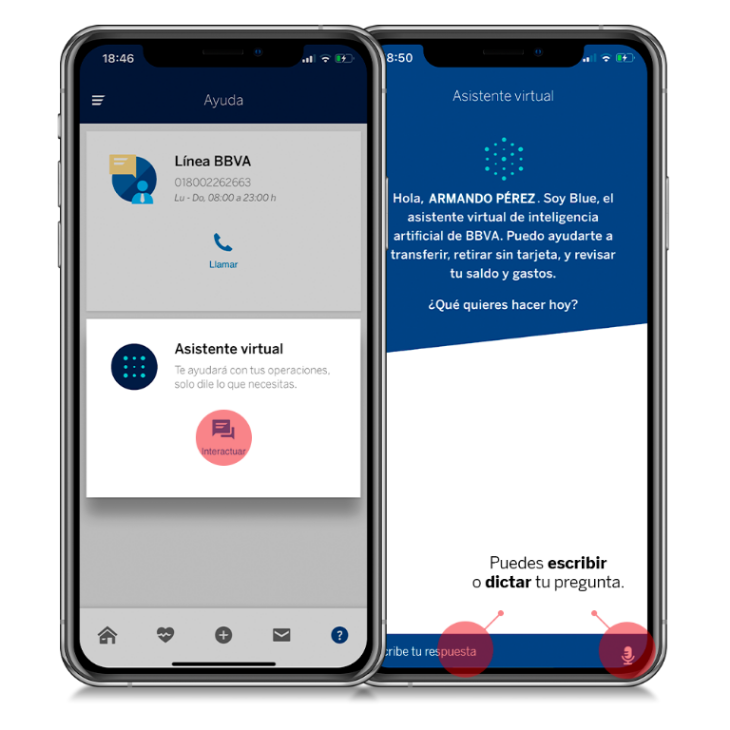
\includegraphics[scale=0.375]{images/1/blue-bbva}
    \caption{Asistente virtual Blue.Fuente: \url{https://www.bbva.com/es/mx/cuatro-funcionalidades-de-blue-para-facilitar-la-vida-de-los-clientes/}}
    \label{fig:blue-bbva}
\end{figure}

Un reporte hecho por la empresa \textit{Reports and Data} estima que la demanda de los chatbots tenga un crecimiento de 30.9\% en el 2026 en comparación a la demanda del año 2019 (figura \ref{fig:demanda-chatbots}) . Esto es porque muchas empresas e instituciones buscan formas de inovar el contacto y divulgación de información a través de un asistente virtual, \textit{queriendo volver obsoleto al modelo actual} de navegación de sitios web como una interfaz a la información; \textbf{es mas factible interactuar con información mediante los chatbots}.

\begin{figure}[ht]
    \centering
    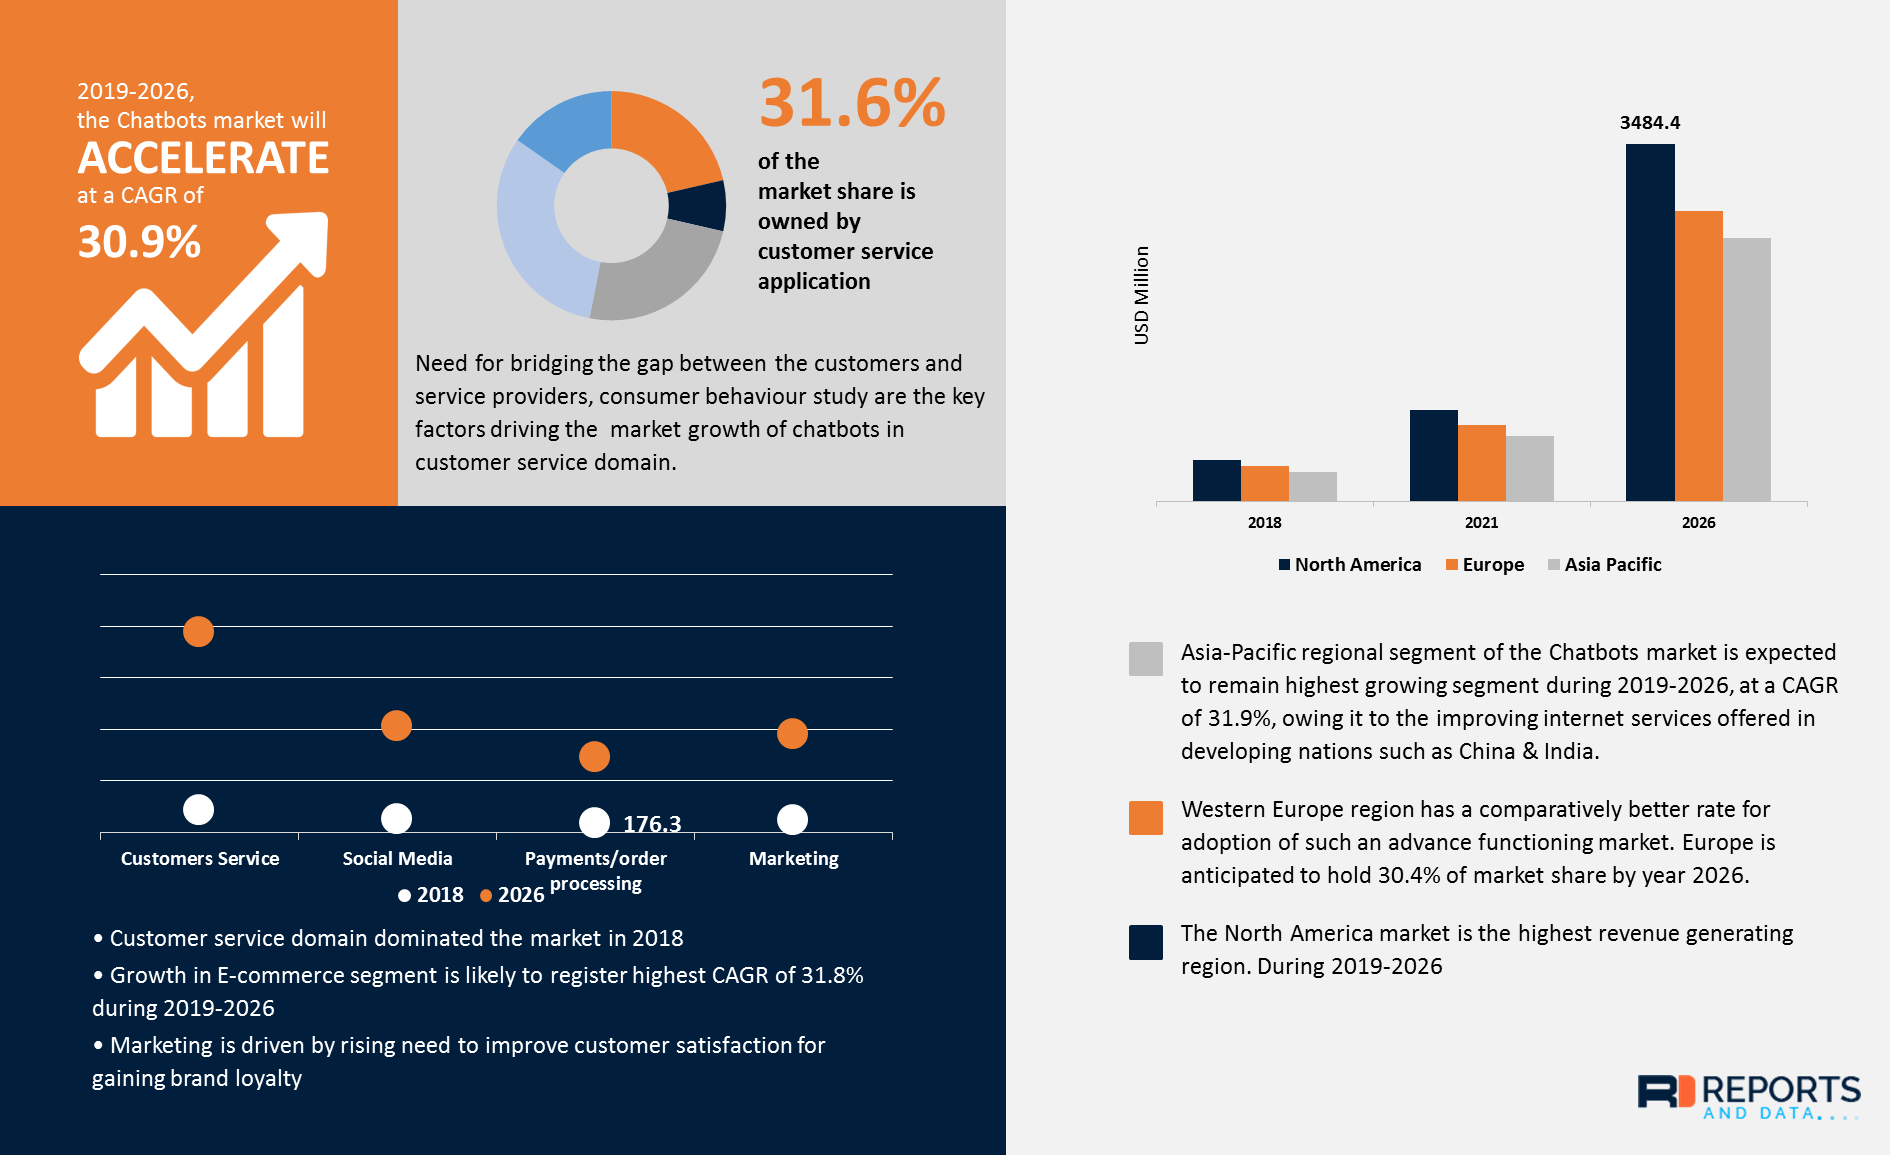
\includegraphics[scale=0.5]{images/1/demanda-chatbots}
    \caption{Fuente: \url{https://www.reportsanddata.com/report-detail/chatbot-market}}
    \label{fig:demanda-chatbots}
\end{figure}

\section{El Uso de un Chatbot Para Orientación Normativa}

\begin{figure}[ht]
    \centering
    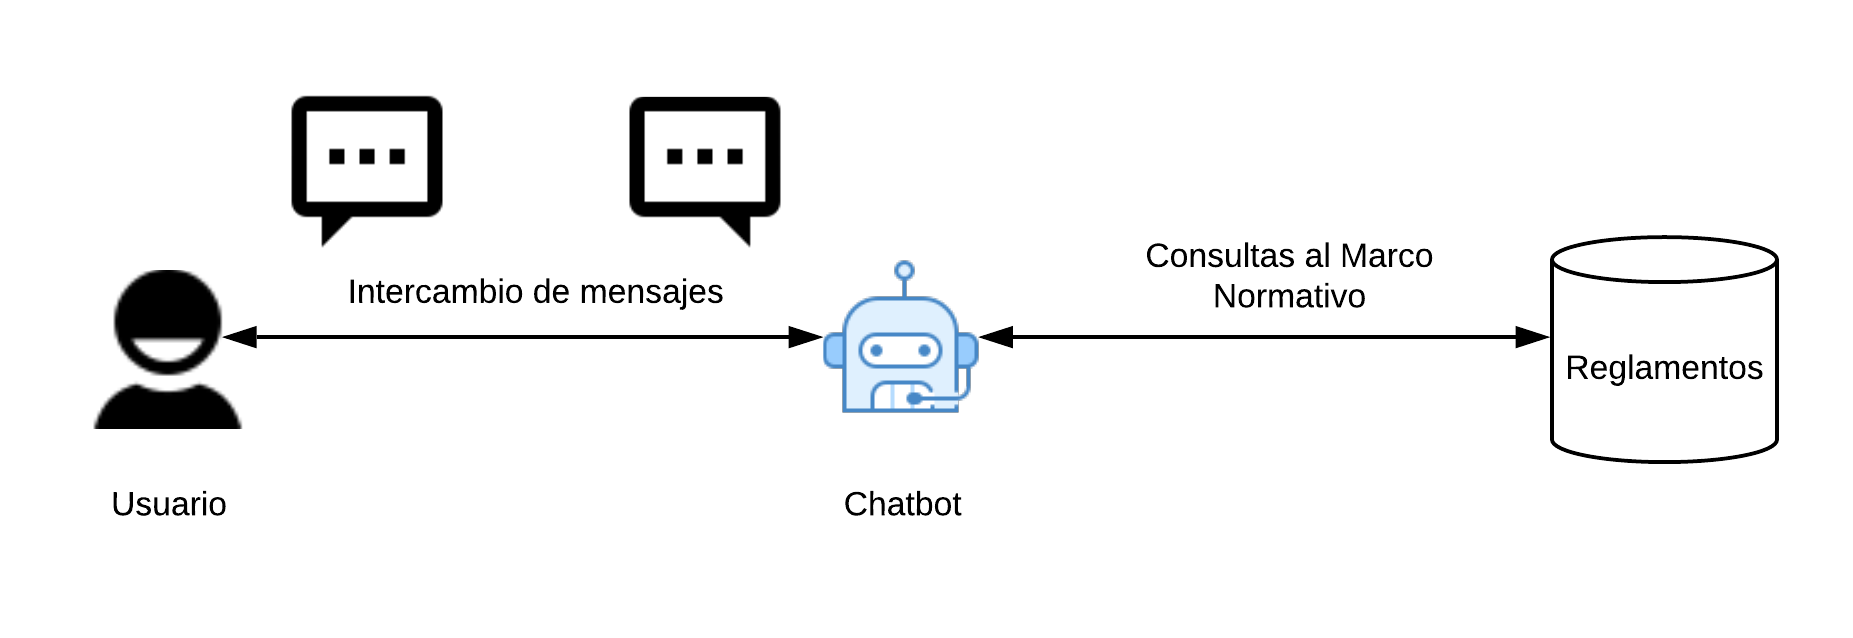
\includegraphics[scale=1]{images/1/propuesta-aplicacion.png}
    \caption{Automatización de una asesoría mediante un chatbot}
    \label{fig:propuesta-aplicacion}
\end{figure}

¿Por qué un chatbot? Una alternativa en la que se podría implementar una solución basada en crear un \textbf{motor de búsqueda}. Esta alternativa podría tener un desarrollo mas sencillo, pero a costo de una interfaz con mas elementos de configuración para el tipo de búsqueda. La compensación de complejidad de desarrollo por una mayor experiencia de usuario mediante el intercambio de dialogo es la principal motivación para decidir implementar la solución mediante un chatbot, ya que un buen diseño conversacional elimina la necesidad de que un usuario configure entradas y parámetros antes de utilizarlo.

Por naturaleza, somos capaces de utilizar el fenómeno de la comunicación para intercambiar información múltiples maneras con el mismo significado, o si no algo similar. En este proyecto aprovecharemos la facilidad de la expresión de diálogo y con ello establecer funcionalidades para cumplir el objetivo propuesto. Contrario a esto, sería que el usuario introduzca de manera rígida de un formulario o la introducción de parámetros de búsqueda.

% Move this to proposal
Adicional a esto, la integración de estos servicios a los portales web del Instituto Politécnico Nacional podrían aprovechar el uso de canales de comunicación. Esto para auxiliar a la comunidad escolar en la obtención de una asesoría previa a la intervención de una persona experta en el tema.
% Intetrate to current communication channels

Este proyecto propone el desarrollo de un chatbot que funcione como sistema de recuperación de información para atender los problemas mencionados. Estará disponible a través de una aplicación web que se pueda utilizar desde un navegador web que funcionará como cliente de este servicio.

\chapter{Marco Teórico}

%
% Parte conceptual
%

\section{Normatividad}

De acuerdo con la Real Academia de la Lengua Española, un \textbf{reglamento} es una norma que rige la organización y funcionamiento de cualquier establecimiento o institución, públicos o privados. \parencite{rae}

\subsection{Marco Jurídico y Marco Normativo}

A continuación se definen los siguientes conceptos.

\begin{quote}
\textbf{Marco Jurídico}: Conjunto de leyes, reglamentos, Conjunto de disposiciones, leyes, reglamentos y acuerdos a los que debe apegarse una dependencia o entidad en el ejercicio de las funciones que tienen encomendadas.. \parencite{riverarobles}
\end{quote}

\begin{quote}
% Change this definition
\textbf{Marco Normativo}: Conjunto general de normas, criterios, metodologías, lineamientos y sistemas, que establecen la forma en que debe desarrollarse su cumplimiento. \parencite{diccionariomarconormativo}
\end{quote}

Para que un reglamento deba ser válido debe tener una base legal y establecer las especificaciones del cumplimiento. Ambos conceptos de marco jurídico y normativo se fundamentan en la necesidad de una base para la regulación de las actividades que se desempeñan de manera colectiva y a nivel individuo.

La unidad atómica de un hecho que establece un enunciado legal es el \textit{artículo}, expresando mediante la misma información de un concepto de manera especifica. Es por esto que estos enunciados forman la base para fundamentar un derecho u obligación. Así mismo, los artículos se dividen de manera estructural agrupando temas de una sola materia.

\subsection{Reglamentos del Instituto Politécnico Nacional}

Como ya se ha mencionado, \textit{el Instituto Politécnico Nacional es un órgano desconcentrado de la Secretaría de
Educación Pública}, que a su vez es una dependencia del gobierno del estado. El IPN tiene su base jurídica a través de su \textit{Ley Orgánica} para regular las funciones científicas y académicas que debe cumplir.

A continuación se muestra una tabla con los 29 reglamentos utilizados en el marco normativo del Instituto Politécnico Nacional y una descripción de la materia normativa que abarca.

\newpage

\begin{tabular}{ | m{17em} | m{25em}|}
    \hline
    \textbf{Reglamento} & \textbf{Descripción} \\
    \hline
    Reglamento de Estudios de Posgrado & Norma el ingreso, permanencia y egreso de los alumnos que cursen alguno de los programas académicos  de  nivel  posgrado, \\
    \hline
    Reglamento Orgánico & Establece  las  bases  de la organización y la distribución de competencias entre las distintas unidades administrativas, académicas y otras dependencias que conforman la estructura orgánico-funcional. \\
    \hline
    Reglamento del Sistema de Becas por Exclusividad & Establece las condiciones y términos para el otorgamiento de becas por exclusividad en el ámbito de competencia para profesores de carrera de tiempo completo clasificado como trabajador base y a los incorporados a través del Programa de Contataciones Extraordinarias. \\
    \hline
    * Reglamento Interior de la Comisión Nacional del Sistema de Ahorro para el Retiro & Define la organización, estructura y facultades de las unidades administrativas de la Comisión Nacional  del  Sistema  de  Ahorro  para  el  Retiro.\\
    \hline
    * Reglamento del Instituto para la Protección al Ahorro Bancario & Establece las unidades administrativas del Instituto para la Protección al Ahorro Bancario. \\
    \hline
    * Reglamento de la Ley sobre Refugiados y Protección Complementaria & Establece las condiciones de refugiado y reglamenta las sus leyes de protección. \\
    \hline
    *Reglamento para la integración y funcionamiento de la Comisión de Apelación y Arbitraje del Deporte & Regular la integración y funcionamiento de la Comisión de Apelación y Arbitraje del Deporte. \\
    \hline
    *Reglamento de la Junta de Gobierno del Consejo Nacional para Prevenir la Discriminación. & Reglamenta la conducción y funcionamiento de la Asamblea Consultiva del Consejo Nacional para Prevenir la Discriminación. \\
    \hline
    * Reglamento de Pasaportes y del Documento de Identidad y Viaje. & Regular la expedición, renovación y cancelación del pasaporte y del documento de identidad y viaje. \\
    \hline
    Reglamento General de Estudios del Instituto Politécnico Nacional. & Establecer las condiciones que regulan el ingreso, la trayectoria escolar, la permanencia y el egreso de alumnos que cursen algún programa académico de los niveles medio superior, superior y posgrado, así como de los usuarios de todos aquellos programas que se ofrezcan.  \\
    \hline
    Reglamento de promoción docente del Instituto Politécnico Nacional. & Regula el proceso de promoción docente. \\
    \hline
    *Reglamento de Becas del Programa de Fomento, Formación, Desarrollo y Vinculación de Recursos Humanos de Alto Nivel del Consejo Nacional de Ciencia y Tecnología. &  Para las instancias encargadas de la conducción y operación del Programa  de Fomento, Formación, Desarrollo y Vinculación de Recursos Humanos de Alto Nivel del CONACyT y para quienes estén recibiendo o pretendan recibir los apoyos o beneficios. \\
    \hline
    Reglamento de Integración Social del Instituto Politécnico Nacional. & Regula las actividades de integración social, sus alcances y objetivos. \\
    \hline
    Reglamento del Consejo General Consultivo del Instituto Politécnico Nacional. & Regular la integración, funcionamiento y organización del Consejo General Consultivo del Instituto Politécnico Nacional. \\
    \hline
    Reglamento del Decanato del Instituto Politécnico Nacional. & Regular el funcionamiento y atribuciones del Decanato como órgano colegiado, de su presidente y de los maestros decanos de cada escuela, centro o unidad de enseñanza y de investigación del Instituto. \\
    \hline
    Reglamento del Archivo Histórico del Instituto Politécnico Nacional. & Otorgar distinciones por el reconocimiento que hace la comunidad politécnica a una conducta, trayectoria, servicios o acciones ejemplares o sobresalientes que hayan tenido por objeto exaltar el prestigio de esta casa de estudios, apoyar la realización de sus finalidades, impulsar el desarrollo de la educación técnica en el país o beneficiar a la humanidad. \\
    \hline
    
\end{tabular}

\begin{tabular}{ | m{17em} | m{25em}|}
    \hline
    \textbf{Reglamento} & \textbf{Descripción} \\
    \hline
    Reglamento de Distinciones al Merito Politécnico del Instituto Politécnico Nacional. &  Fijar las relaciones entre el personal docente de Educación Media Superior y de Educación Superior del Instituto Politécnico Nacional y el Programa de Estímulo al Desempeño Docente. \\
    \hline
    Reglamento del Programa de Estímulo al Desempeño Docente del Instituto Politécnico Nacional. & Fijar las relaciones entre el personal docente de Educación Media Superior y de Educación Superior del Instituto Politécnico Nacional y el Programa de Estímulo al Desempeño Docente. \\
    \hline
    Reglamento Interno del Instituto Politécnico Nacional. & Establecer lineamientos metodológicos básicos de la reforma reglamentaria el mantener y respetar estrictamente lo establecido en la Ley Orgánica. \\
    \hline
    Reglamento Interior de la Comisión de Operación y Fomento de Actividades Académicas del Instituto Politécnico Nacional. & Establecer los reglamentos  para el cumplimiento del objetivos del COFAA como Organismo Público Descentralizado y Entidad  de  la  Administración  Pública  Paraestatal. \\
    \hline
    Reglamento de Titulación Profesional del Instituto Politécnico Nacional. & Establecer las normas para el otorgamiento de títulos profesionales a los pasantes del Instituto Politécnico Nacional y de sus planteles incorporados.  \\
    \hline
    Reglamento de Evaluación del Instituto Politécnico Nacional. & Regular  la  función  de  evaluación  que  se  desarrolla  en  el  Instituto  Politécnico  Nacional. \\
    \hline
    Reglamento de Academias del Instituto Politécnico Nacional. & Establecer normas para la integración y funcionamiento de las academias de profesores en las escuelas,  centros y unidades de enseñanza. \\
    \hline
    Reglamento de Planeación del Instituto Politécnico Nacional. & Establecer las normas y principios básicos para la integración y funcionamiento del Sistema Institucional de Planeación. \\
    \hline
    Reglamento de Prácticas y Visitas Escolares del Instituto Politécnico Nacional. & Establecer las normas a las que se sujetarán las prácticas o visitas escolares que realicen los alumnos y pasantes del IPN. \\
    \hline
    Reglamento de las Condiciones Generales de Trabajo del Personal no Docente del Instituto Politécnico Nacional. &  Fija las Condiciones de Trabajo del Personal No Docente del Instituto Politécnico Nacional, que conjuntamente con sus dos anexos. \\
    \hline
    Reglamento del Patronato de Obras e Instalaciones del Instituto Politécnico Nacional. & Establece las normas a las que se sujetan el Patronato de Obras e Instalaciones del Instituto Politécnico Nacional como órgano público descentralizado. \\
    \hline
    Reglamento de las Condiciones Interiores de Trabajo del Personal Académico del Instituto Politécnico Nacional. &  Fija las condiciones de trabajo del personal académico del Instituto Politécnico Nacional. \\
    \hline
    Reglamento del Centro Nacional de Cálculo. & Establece las normas para los procesos profesionales y actividades de investigación del Centro Nacional de Cálculo. \\
    \hline
\end{tabular}

%
% Parte conceptual
%

\section{Inteligencia Artificial}

La inteligencia artificial es un conjunto multidisciplinario de ciencias y filosofías basados en el principio de la simulación de la inteligencia humana, la mas compleja observada hasta ahora. Abarca una variedad amplia de aspectos que podrían considerarse dentro de un \textit{comportamiento mediante el razonamiento}, tales como maquinas que se conduzcan solas o algoritmos que puedan optimizar decisiones basadas en pronósticos obtenidos mediante aprendizaje. \parencite{russelnorvig}.

Los algoritmos que implementan esta inteligencia añaden mas valor cuando intentan asimilar una función desconocida para poder acercarse a un comportamiento que reproduzca esos resultados. A esto se le conoce como \textbf{aprendizaje automático} y generalmente se dividen en dos categorías: \textit{supervisado} y \textit{no supervisado}. \parencite{murphypkevin}

% \subsection{Aprendizaje Automático Supervisado}

% Esta forma de aprendizaje está basada en el enfoque predictivo basado en el estado de la entrada a una función. Esto requiere construir un modelo mediante una población de datos de entrada y otra población de datos que implican que fueron obtenidos a base de la entrada. El objetivo es poder mapear una entrada $\mathbf{x}$ a una salida $y$, dado un conjunto de datos de entrenamiento en forma de tupla entrada-salida:

% $$
% D = \{\mathbf{x_i}, y_i\}^N_{i=1}
% $$

% La figura \ref{fig:iris-classification} muestra como se clasifican tipos de flores iris de acuerdo usando \textit{machine learning}. De esta forma se busca encontrar un modelo de clasificación que esté en función de los atributos de la entrada.

% \begin{figure}[ht]
%     \centering
%     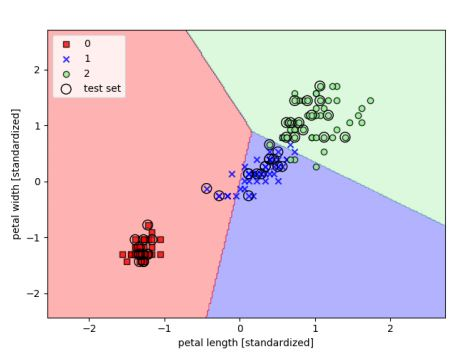
\includegraphics[scale=0.75]{images/2/iris-classification}
%     \caption{Clasificación un conjunto de datos de flores iris.}
%     \label{fig:iris-classification}
% \end{figure}

% \subsection{Algoritmo K-Means}



% Esto es especialmente útil en aplicaciones como chatbots porque queremos que \textbf{la intención del usuario esté en función del mensaje que escribe}. Por ejemplo, algunas intenciones y ejemplos de mensajes son:

% \begin{itemize}
%     \item \textbf{Saludar}:
    
%     \begin{enumerate}
%         \item \textit{Hola.}
%         \item \textit{Buenos días.}
%         \item \textit{Buenas tardes.}
%     \end{enumerate}
    
%     \item \textbf{Solicitar Reglamento}
    
%     \begin{enumerate}
%         \item \label{itm:intencion-solicitar}\textit{Dime qué dice el \textbf{artículo 3} de la \textbf{Ley Orgánica}}.
%         \item \textit{¿Qué dice el \textbf{artículo 9} del \textbf{Reglamento General de Estudios}?}
%     \end{enumerate}
% \end{itemize}

% La idea es que con base a un conjunto de entrenamiento de mensajes ejemplo podamos \textit{clasificar la intención}. Además, una vez identificada la intención también pueda clasificar a \textbf{entidades} de interés para saber qué información se está solicitando. Por ejemplo, el ejemplo \ref{itm:intencion-solicitar} de la intención de solicitar reglamento requiere reconocer que se está pidiendo el \textbf{artículo} un \textbf{documento}, por lo que son dos entidades que el chatbot debe aprender en ese ejemplo. 

% Cuando se trata de texto, por lo regular se utilizan \textbf{redes neuronales recurrentes}, que aprenden con base a una secuencia de valores.

\section{Procesamiento de lenguaje natural}

El lenguaje natural es un fenómeno lingüístico que abarca la creación y constante evolución del lenguaje que los humanos obtienen a través del uso ordinario y cotidiano en el uso de la comunicación formal. El lenguaje natural es la forma mas sencilla en la que se codifica conocimiento a través de hábitos cognitivos pero a la vez complejo debido a que la inteligencia humana no tienen forma estructurada de comprenderse.

El procesamiento de lenguaje natural, también conocido como \textit{lingüística computacional}, es una aplicación de la inteligencia artificial enfocada a crear entidades que puedan simular la inteligencia humana con capacidades de entendimiento y síntesis de lenguaje natural o humano. La \textit{lingüística} es el estudio científico del lenguaje que se encarga de estudiar múltiples aspectos del lenguaje y funciona como una base estructurar elementos de un lenguaje en componentes o unidades dependiendo el tipo de análisis.

Uno de las unidades mas comunes es una \textbf{palabra} la cual puede derivar significado por si solo. Posteriormente, existen categorías para clasificar palabras, como lo son \textit{sustantivos}, \textit{verbos}, \textit{adjetivos}, \textit{adverbios}, entre otras menos comunes. \parencite{dipanjan}.

Estas palabras forman grupos para agregar significado mediante \textit{frases} o \textit{cláusulas}, que a su vez pueden estructurarse mediante gramáticas que describan las relaciones entre esos grupos de palabras. Para propósitos de este proyecto, inicialmente tomaremos al conjunto de palabras en oraciones para derivar un significado.

\subsection{Semántica}

Entre los objetos de estudio de la lingüística está la \textbf{semántica}, la cuál envuelve el estudio del \textit{significado}. Por sí solo, la semántica es una teoría compleja que abarca cuestiones un tanto filosóficas y hasta metafísicas, no tanto del significado mismo de las palabras sino la causa del \textit{por qué las palabras tienen significado}. Teorías de la semántica deben contestar las preguntas de \textit{cuál es la naturalez del significado} o \textit{qué produce en nuestro conocimiento cuando conocemos un significado de una palabra} \parencite{sep-word-meaning}.

Para poder procesar significado, se puede subdividir en dos categorías para entender sus componentes \parencite{dipanjan}. Estas son:

\begin{itemize}
    \item \textbf{Semántica léxica}: El estudio del significado de las palabras y símbolos usando morfología y sintaxis.
    \item \textbf{Semántica composicional}: Estudia las relaciones entre las palabras y la combinación de las mismas que constituyen un significado a través de frases y oraciones.
\end{itemize}

Mientras que un ser humano tiene la capacidad de procesar significado de una manera casi inmediata,  resulta ser complejo representar un proceso de \textit{extracción de significado} para una computadora. Hasta la fecha estos problemas solo pueden ser resueltos delimitando el dominio del lenguaje a un uso específico y utilizando \textit{modelos de aprendizaje automático supervisados}, los cuáles obtienen como datos de entrenamiento un grupo de palabras y meta información y otro grupo del "significado representativo que deben tener". Esta abstracción debe poder cuantificarse de alguna manera para poder procesarlo y automatizarlo mediante inteligencia artificial.

Una de las formas mas básicas de representar semántica uniforme es utilizando \textbf{lemas} o \textbf{lematización de palabras}. Un lema es una forma canónica de las palabras. Forma una unidad base para derivar significado dependiendo de las múltiples inflecciones de le base. Un ejemplo común de esto es la conjugación de verbos.

\subsection{Sistemas de Recuperación de Información de Texto}

Regularmente, mucha de nuestra información en el lenguaje español se transmite y se almacena en algún formato textual (e.g., libros, revistas, diccionarios, artículos, publicaciones, conversaciones, etc.). Todo eso se puede almacenar en un repositorio de información para un uso posterior. A esto se le conoce como \textbf{corpus de texto} Pero por si solo, el texto no es suficiente para ser de alguna utilidad, sino lo que significa todo o alguna porción del texto. Entre mas grande crece el corpus de texto, mas dispersa se vuelve la información y mas significado se puede sacar de manera acumulada.

Una de las aplicaciones útiles del procesamiento de lenguaje natural es precisamente el utilizado en este proyecto: la \textbf{recuperación de información} o \textbf{information retrieval} en inglés. La recuperación de información se define como un actividad de obtención de información relevante de una fuente de datos. Estos sistemas son muy útiles debido a que una información relacionada, que puede significar lo mismo o estar muy relacionado pero varía en morfología, e incluso hasta de idioma. Para propósitos de este proyecto, haremos nuestro enfoque la información textual en español para poder dar solución al problema establecido en el capítulo 1.

La forma en que esta recuperación se lleva a cabo es un caso de estudio en su propia cuenta. Puede ser desde la búsqueda idéntica de valores hasta métodos probabilísticos que infieren una similitud semántica de la información. Generalmente estos métodos utilizan una \textbf{función de similitud}, la cual opera sobre un \textbf{espacio vectorial} que contiene información textual. La transformación de un palabra o conjunto de palabras a un vector de palabras se le conoce como \textbf{word embedding} (incrustación de palabras). Mediante esta representación vectorial es posible cuantificar que tan parecidos son dos vectores de palabras o \textit{word embeddings}. \parencite{zhaimassung}.

\begin{figure}[ht]
    \centering
    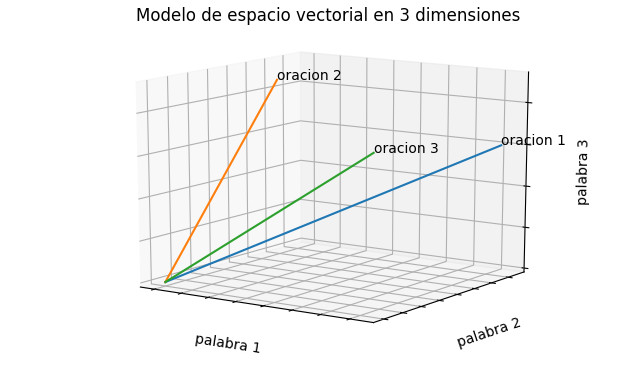
\includegraphics[scale=0.6]{images/2/vector-space-model}
    \caption{Representación gráfica de un vocabulario de 3 palabras sobre un espacio vectorial de $\mathbb{R}^3$.}
    \label{fig:espacio-vectorial}
\end{figure}

La dimensión de este espacio vectorial es determinada por el tamaño del conjunto en el vocabulario de palabras que se usarán en un modelo lingüístico. La figura \ref{fig:espacio-vectorial} muestra un ejemplo de un espacio vectorial de 3 dimensiones con las que se pueden construir oraciones; los vectores en la gráfica son oraciones y se les conoce como \textbf{vectores de palabras}. Bajo esta representación vectorial se pueden ejecutar operaciones matemáticas para cuantificar qué tan similar son estas oraciones en el espacio.

Por ejemplo, si la entrada es una consulta transformada a un vector de palabras $\vec{q}$ buscaremos trasladar esta consulta en el espacio vectorial y observar qué vectores cercanos se encuentran al de la consulta; entre mas cercanos, mas relevantes serán. Una función de similitud entre vectores muy conocida es la \textbf{similitud coseno}. 

Sean 

$$\vec{a},\vec{b} : \text{vector de } n \text{ dimensiones correspondiente a una oración.}$$

Entonces, la similitud entre esas dos oraciones se puede calcular mediante la fórmula:

$$
sim(\vec{a}, \vec{b}) = \frac{\vec{a} \dot \vec{b}}{\| \vec{a} \| \| \vec{b} \|}
$$

Estos vectores se pueden construir de múltiples maneras: mediante usos de aprendizaje automático representados como $\vec{w} = (w_0, w_1, ..., w_n)$ en donde $w_i$ pertenece a un vocabulario $\mathbf{V}$. Algunas formas de representación de vectores son:

\begin{itemize}
    \item \textbf{Representación de bits}: una forma sencilla y rápida de representar un conjunto de palabras es indicando si esa palabra está presente o no. Matemáticamente, el vector se calcula de la siguiente manera:
    
    \begin{equation*}
        a(i) = 
        \begin{cases}
            1 & \text{si la palabra está presente en la oración}\\
            0 & \text{en otros casos}
        \end{cases}
    \end{equation*}

    \item \textbf{Representación basados en frecuencias}: Dada una colección de documentos se puede utilizar varios factores para determinar significado de un conjunto de palabras en cuánto al dominio de esos documentos, como la frecuencia de las veces que aparece en el documento y en cuántos de ellos aparece. Derivado de eso se puede refinar aún mas normalizando palabras que se utilizan de manera excesiva y destacar palabras poco frecuentes como mas significativas. 
    
    Sea
    
    \begin{align*} 
        q: & \text{ una oración correspondiente a una consulta}\\
        d: & \text{ un documento}\\
        M: & \text{ la cantidad de documentos}\\
        c(w, q): & \text{ función que cuenta las ocurrencias de } w \text{en } q\\
        df(w): & \text{ cantidad de documentos que contienen a } w
    \end{align*}
    
    Entonces una oración cosulta $q$ puede ser representada mediante la siguiente fórmula:

    $$
    f(q, d) = \sum_{w \in q \cup d} c(w, q) c(w, d) log \frac{M + 1}{df(w)},
    $$
\end{itemize}

\subsection{Algoritmo de Detección de Paráfrasis}
\label{sec:deteccion-parafrasis}

Para este proyecto usaremos un método llamado detección de paráfrasis, el cual consiste en buscar una forma de relacionar las palabras utilizadas en la consulta y obtener los segmentos de texto en los reglamentos del marco normativo. De esta manera evitamos búsquedas de palabras exactas cuando podrían encontrarse como un sinónimo. Este algoritmo fue presentado por \cite{fernando2008semantic}.

En primera instancia, se debe considerar un espacio vectorial que abarque la mayor cantidad de palabras posibles, pero entrenando su semántica lo mas cercano posible al tema o dominio de interés. Por ejemplo, \textbf{Spacy} proporciona un modelo entrenado utilizando el algoritmo \textbf{word2vec} (\url{https://github.com/explosion/spacy-models/releases/tag/es_core_news_md-2.2.5}) para el lenguaje español. 

Una vez obtenido este espacio, se debe representar las palabras en su forma vectorial y utilizar la similitud coseno para construir una matriz $\mathbf{W}$, la cuál representa todas las similitudes posibles que existen en el vocabulario. Cabe mencionar que la matriz resultante es una matriz cuadrada cuya condición $\mathbf{W}_{i,j} = 1$ cuando $i = j$; es decir, una palabra es similar a sí misma.

$$
\mathbf{W}_{i,j} = sim(w_i, w_j)
$$

Supongamos entonces que un usuario introduce una consulta $\vec{q}$, la cuál es una oración compuesta de palabras utilizando el mismo vocabulario. Queremos comparar esta consulta con segmentos de texto $\vec{s}$ para calcular su relevancia. Esto se hace con la siguiente fórmula:

$$
sim(\vec{q}r, \vec{s}) = \frac{ \vec{q^T} \mathbf{W} \vec{s}}{\| \vec{q} \|  \| \vec{s} \|}
$$

Los vectores $\vec{q}$ y $\vec{s}$ son vectores binarios indicando la presencia de una palabra. Como cada palabra constituye una dimensión en este espacio vectorial, estos vectores debemos representarlos como la suma de los vectores unitarios que representan las palabras presentes en la oración. Si $\vec{a}$ se obtiene a partir de una oración, entonces a se obtiene de la siguiente forma:

$$
\vec{a} = 
\begin{pmatrix}
    a_0\\
    a_1\\
    a_2\\
    \vdots \\
    a_n
\end{pmatrix}
$$

\begin{equation*}
a(i) = 
    \begin{cases}
        1 & \text{si la palabra está presente en la oración}\\
        0 & \text{en otros casos}
    \end{cases}
\end{equation*}

Esto hace que solo se calculen las similitudes de las palabras presentes en la consulta y en el texto a comparar, mientras que se ignorar palabras que no están presentes.\textbf{}

\subsection{Preparación de los datos}

Para poder operar consultas con este método, necesitamos lo siguiente:

\begin{enumerate}
    \item Los vectores de las palabras deberán remover \textit{palabras vacías} (artículos, pronombres, preposiciones, etc.).
    \item Las palabras resultantes utilizarán en su forma \textit{lematizada}.
    \item \label{itm:matriz-w} La matriz de similitud $\mathbf{W}$ deberá estar calculada previamente.
\end{enumerate}

\subsection{Métricas Adicionales de Semántica}

El uso exclusivo de una matriz de similitud considera un nivel básico de parafraseo por la mera presencia de palabras en un enunciado, o en su defecto algunas similares. Sin embargo, hay algunos factores adicionales que agregan sentido estructural en cuanto a como se relacionan los conceptos. \parencite{batetsanchesvalls2010semantic}

\begin{figure}
    \centering
    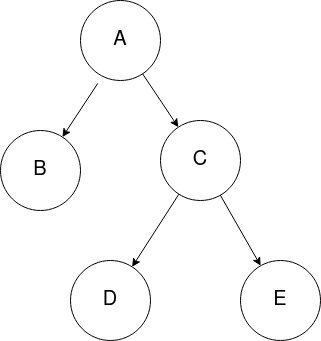
\includegraphics[scale=0.5]{images/2/arbol-simple}
    \caption{Arbol de entidades. Cada nodo representa una entidad mientras que los vértices representan relaciones entre ellos.}
    \label{fig:arbol-entidades}
\end{figure}


Se puede medir el nivel de cercanía en una estructura taxonómica basada en clases ontológicas de su significado. Por ejemplo, agregar una jerarquía de entidades como \textbf{PERSONA} derivando a \textbf{ESTUDIANTE}, la cual puede tener mas clases dependiendo del dominio que deba especificar. En este caso la estructura resultante sería una similar al de la figura \ref{fig:arbol-entidades} y la distancia implicada es la profundidad.


En ese caso, existe una red semántica de entidades conectadas por vértices que implican una relación entre ellas, las cuales se pueden medir con distancias para denotar similitud:

$$
d(c_1, c_2) = \text{Menor cantidad posible de vértices conectando a } c_1 \text{ y } c_2
$$

La ecuación exacta varía dependiendo de los factores a considerar y de la complejidad que se busca. Varias propuestas se pueden encontrar en \cite{batetsanchesvalls2010semantic}.

\chapter{Estado del arte}

Los chatbots funcionan como asistentes virtuales que automatizan procesos determinados. Por lo regular este servicio de asistencia es atendido por una persona que es capaz de comunicarse con un cliente que se presenta con un problema en específico. La esencia principal de los chatbots es la automatización de esta interacción con clientes. Sin embargo, el problema que trata de atender es un asunto que se debe delimitar a un proceso de solución que esté a la medida.

Dicho eso, cabe mencionar que sería difícil generalizar todos los problemas y automatizar un proceso que los solucione todos. Por lo tanto, dependiendo de la necesidad de los usuarios de un servicio, se encontrará que existen diversos chatbots que atienden necesidades muy específicas.

\section{Chatbots Para Asesoría Jurídica}

Dentro del ámbito jurídico y normativo, existen chatbots que automatizan servicios de asesoría. Un ejemplo de esto es \textbf{Ailira: Artificially Intelligent Legal Information Research Assistant} (\url{https://www.ailira.com/australian-tax-research/}), un bot. Este bot es una herramienta útil para la investigación en materia fiscal. Proporciona una manera para solicitar información de casos y determinaciones anteriores, así como una forma de investigación de leyes fiscales australianas.

Otro chatbot que funciona para la asesoría e investigación de materia legal es \textbf{Parker: Insurance} (\url{https://www.nortonrosefulbright.com/en/knowledge/publications/58422d30/welcome-to-parker-insurance}). Su propósito es ayudar a los usuarios a responder preguntas acerca de IDD (Insurance Distribution Directives) Europea, o directivas de distribución de seguros. Brinda una asesoría que otorga definiciones normativas, requerimientos y cómo se aplican en cuestiones de la IDD.

La materia normativa y legislativa que ambos sistemas manejan está fuera del alcance de este documento. Sin embargo, es suficiente mencionar que el uso de chatbots para asesoría normativa no es algo nuevo.

Cabe mencionar que ambos son aplicaciones proporcionado por un tercero, del cuál su uso no está abierto al público en general, ya que se requiere agendar una demostración para su posterior adquisición. Esto ha dificultado la demostración de las características de ambos y realizar una comparativa entre ellas y la propuesta de este proyecto.

% \section{Herramientas de diseño para chatbots}

% En la actualidad, existen algunas herramientas para construcción de aplicaciones de chatbots enfocados a transformar un proceso transaccional dentro de un negocio a una conversación. Algunos procesos son agendar una cita con un médico, ordenar una pizza, realizar operaciones bancarias, entre otras.

% Josef (\url{https://joseflegal.com/}), un chatbot para uso legal que automatiza los procesos de atención a los posibles clientes. Permite agilizar el manejo de peticiones y aumenta la experiencia para los usuarios al obtener información previa al trato directo. De esta manera, la preparación previa al trato directo es menor al poder generar documentos y contratos personalizados.

% \begin{figure}[ht]
%     \centering
%     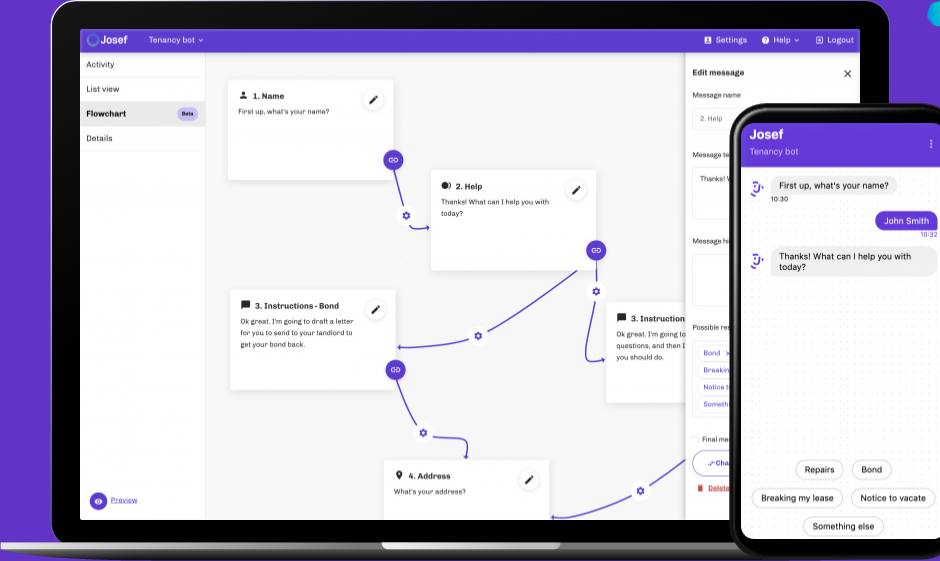
\includegraphics[scale=0.4]{images/3/chatbot-josef}
%     \caption{Ejemplo de una aplicación desarrollada en Josef}
%     \label{fig:josef}
% \end{figure}
    
% También existe TARS. (\url{https://hellotars.com/chatbot-templates/}). Es una herramienta de publicidad y marketing para construir chatbots en landing pages. Su propósito es proporcionar un aumento en la experiencia a posibles clientes mediante una conversación en lugar de contenido estático que debe ser leído. Sin embargo, esta herramienta proporciona plantillas que se pueden personalizar para cierto tipo de servicio; por ejemplo, se puede utilizar para proporcionar asesoría relacionada a la salud y terapia. La plantilla se puede utilizar para los pacientes que sufren depresión y ansiedad, manteniendo al tanto a su doctor de los síntomas que va presentando. Esto agiliza la recolección de información suficiente para los pacientes y transmite información preventiva en caso de requerir ayuda inmediata.

% \begin{figure}[ht]
%     \centering
%     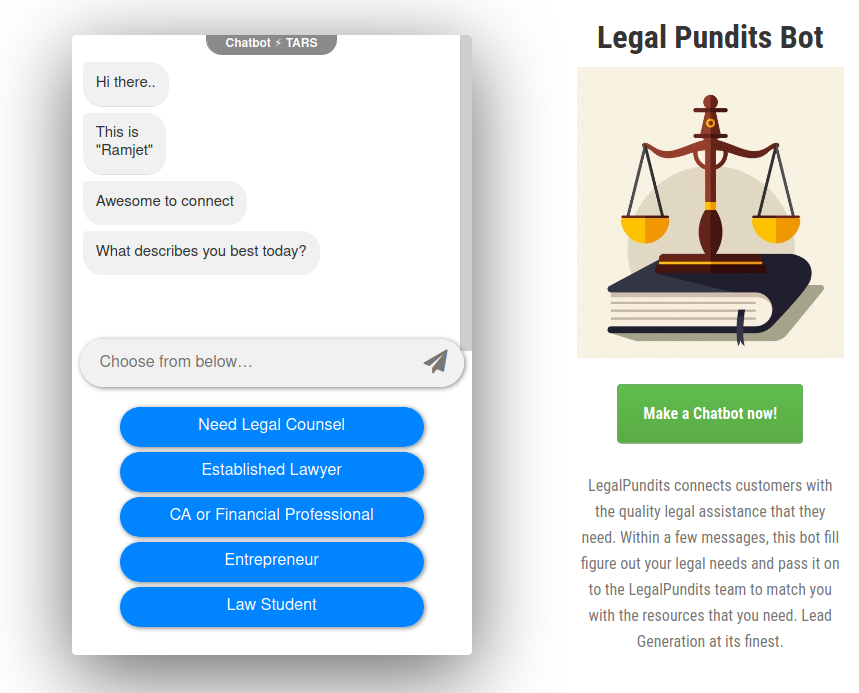
\includegraphics[scale=0.4]{images/3/chatbot-tars}
%     \caption{Plantilla de desarrollo de TARS}
%     \label{fig:tars}
% \end{figure}
    
% HaRi-Bot (\url{https://www.humanresourcesintelligence.com/}) es un chatbot desarrollado para la automatización de las operaciones de los departamentos de recursos humanos de una empresa. El objetivo de este software es el de reducir el tiempo que le toma al departamento de recursos humanos atender preguntas de los empleados, que podrían tomar desde días hasta una semana. HaRi-Bot ayuda a resolver esas que podrían consistir desde políticas internas de la empresa o en procesos administrativos.  

% \section{Librerías y APIs Para Desarrollo de Chatbots}

% Una alternativa atractiva es el de \textbf{Dialogflow} \url{https://dialogflow.com/}, el cual es un API proporcionado por Google para el desarrollo de aplicaciones que usen procesamiento de lenguaje natural. Sin embargo, depende mucho del servicio de \textbf{Google Cloud Platform}, por lo que no permitirá escalar el proyecto sin tener que considerar siempre la oferta de servicios de nube de un solo proveedor.

\section{Librerías y APIs Para Desarrollo de Chatbots}

La necesidad de automatizar un chatbot requiere que se resuelva lo siguiente:

\begin{itemize}
    \item Se debe estructurar bien el formato del conocimiento que el chatbot utiliza.
    \item La manera en que el proceso se lleva a cabo es demasiado específico al problema a resolver.
\end{itemize}

Se puede concluir entonces con estos puntos que para poder cumplir con el objetivo en mente, es necesario desarrollar una aplicación cuya solución esté a la medida del objetivo: el de informar acerca de los reglamentos del Instituto Politécnico Nacional. El estado del arte actual de aplicaciones no están enfocadas con el objetivo de este proyecto.

Es por eso que se hará énfasis en el estado de arte de tecnologías que hacen posible la construcción de chatbots: un conjunto de herramientas para el desarrollo de aplicaciones que implementen algoritmos de inteligencia artificial con filosofía \textit{open source} y licencia abierta. 

Esto permite una gran libertad en el desarrollo de ideas que tengan un impacto benéfico para la comunidad politécnica de la ESCOM; sobre todo la capacidad de poder reclamar el producto final para el bien que se vea conveniente.

Para ello, se presentan a continuación el conjunto de herramientas que ayudan a construir asistentes virtuales:

\begin{figure}[ht]
    \centering
    \begin{tabular}{c c}
        
\includegraphics[scale=0.7]{images/3/python.png} & 
\includegraphics[scale=0.5]{images/3/rasa.png} \\
        
\includegraphics[scale=0.2]{images/3/spacy.png} & 
\includegraphics[scale=0.5]{images/3/numpy.png}
    \end{tabular}
    \caption{Herramientas de desarrollo open source.}
    \label{fig:open-source}
\end{figure}

\subsection{Python}

Un lenguaje de programación de alto nivel que ha tenido una alza de popularidad de uso en áreas como cómputo científico, inteligencia artificial y desarrollo web. Tiene una comunidad extensa, por lo que continuamente existe soporte para el desarrollo de aplicaciones que requieran soporte a largo plazo.

\subsection{Rasa SDK}

Desarrollado y proporcionado por una organización, quienes ofrecen servicios de desarrollo de aplicaciones para asistentes virtuales como chatbots, Rasa SDK es un kit de desarrollo de software (o SDK por sus siglas en inglés) de código abierto soportado por la organización Rasa y la comunidad abierta de desarrolladores.

Facilita la tarea de diseño conversacional con métodos de machine learning, al igual que la integración a servicios web que funcionen como canales de comunicación. Esto con el propósito que el chatbot no solo usarse en un cliente específico como una página web, sino que se pueda integrar a servicios externos como \textit{Facebook Messenger} o \textit{Slack}.

\subsection{Spacy}

Spacy es una biblioteca de funcionalidades dedicadas al procesamiento de lenguaje natural. Contiene algoritmos para procesar texto así como modelos lingüisticos complejos para varios idiomas, entre ellos el español. Su forma de poder procesar texto permite facilmente enfocarse a la lógica de algoritmos de procesamiento de lenguaje natural quitando el peso de encima de procesar cadenas de texto.


\subsection{Numpy}

Esta biblioteca proporciona un conjunto de funciones que optimizan el manejo de memoria para colecciones de datos. Esto es especialmente útil cuando esas colecciones son grandes y requiere computo extenso. Las optimizaciones sobre memoria y el procesamiento sobre ella ha encontrado sus usos en cálculo de operaciones vectoriales y matriciales.
\chapter{Análisis}
% Planeacion del sistema
% Siguiente capitulo: Primer prototipo - Desarrollo Frontend
%   - Analisis
%   - Diseno
%   - etc...

\section{Alcance}

La magnitud de este problema abarca a todos los organismos, direcciones o cualquier dependencia del Instituto Politécnico Nacional. Aunque la solución puede escalar a todo el instituto y su marco normativo, el alcance de este proyecto \textit{considerará únicamente a la comunidad de la Escuela Superior de Cómputo y a los reglamentos con mayor relevancia para las actividades académicas}. Para ello, en este proyecto, inicialmente contará con los siguientes 

\begin{itemize}
    \item Ley Orgánica
    \item Reglamento Interno
    \item Reglamento de Titulación
    \item Reglamento General de Estudios
\end{itemize}

\section{Requerimientos Funcionales}

A continuación, se describe el comportamiento y la funcionalidad esencial para que el chatbot pueda cumplir el objetivo:

\begin{enumerate}[leftmargin=2.5cm ,label={\bfseries RF-\arabic*}]
    \item \label{itm:consultar-reglamento} Un usuario de esta aplicación debe poder consultar un segmento de los documentos del marco normativo en cualquiera de los siguientes niveles de división estructural del documento:
    \begin{itemize}
        \item título
        \item capítulo
        \item sección
        \item artículo.
    \end{itemize}
    
    \item La aplicación debe manejar una conversación de manera lógica (i.e., responder adecuadamente a la conversación en los temas a las preguntas referentes al marco normativo).
    \item \label{itm:requisito-intenciones} El chatbot debe poder detectar si la intención del mensaje es alguno de los siguientes:
        \begin{itemize}
            \item Saludar.
            \item Solicitar información de un articulo.
            \item Solicitar artículos relacionados a una situación en particular.
            \item Despedir.
        \end{itemize}
    \item El chatbot debe saludar de acuerdo a la hora del día.
    \item El chatbot debe poder identificar las entidades o conceptos que el usuario solicita consultar.
    \item \label{itm:rf-servicio-web} La aplicación debe ser disponible a través de un servicio web.
    \item  \label{itm:cliente-web} La aplicación debe proporcionar un cliente accesible a través de un navegador web.
\end{enumerate}

\section{Requerimientos No Funcionales}

\begin{enumerate}[leftmargin=2.5cm ,label={\bfseries RNF-\arabic*}]
    \item Se sugiere que el resultado de las consultas sean breves y concisos. 
    \item El bot debe poder expresar intenciones de asesorar en temas referentes al marco normativo.
    \item Se desea que la aplicación se desarrolle utilizando herramientas de licencia abierta y software libre.
\end{enumerate}


\section{Metodología}

Las actividades a desarrollarse se harán siguiendo una metodología de \textbf{prototipado evolutivo}. Esta elección se hace con base a la necesidad de estar tener que estar evaluando constantemente el diseño inicial de la funcionalidad, principalmente la ejecución del algoritmo de similitud. Para ello, se busca poder refinar detalles sin perder la estabilidad de las iteraciones pasadas.

Los prototipos están basado en los siguientes componentes:

\begin{itemize}
    \item \textbf{Interfaz de usuario}: contiene la página web y el sistema cliente que se encarga de realizar peticiones HTTP al chatbot.
    \item \textbf{Base de conocimiento}: serialización y persistencia del conocimiento de los documentos normativos y su representación semántica necesaria para poder procesarla.
    \item \textbf{Intérprete semántico}: componente de entendimiento del chatbot que se encarga de procesar consultas textuales en búsquedas de similitud sobre la base de conocimiento.
    \item \textbf{Preprocesador de Texto}: contiene todos los ejecutables y las implementaciones de los algoritmos que ayudan a transformar documentos de un formato a otro para la extracción, transformación de datos necesarios para el intérprete y carga a la base de conocimiento.
\end{itemize}

\begin{figure}
    \centering
    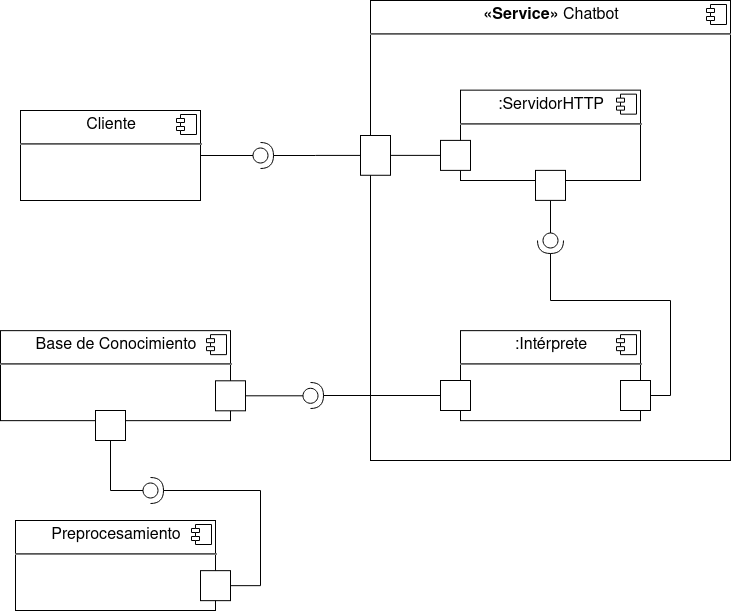
\includegraphics[scale=0.5]{images/4/componentes}
    \caption{Diagrama de componentes}
    \label{fig:diagrama-componentes}
\end{figure}

\subsection{Primer Prototipo}

En este primer prototipo inicial se espera construir el componente visual del  cliente web así como la preparación de los datos a procesar y la definición inicial del esquema en la fuente de datos. Las actividades principales en esta etapa son:

\begin{itemize}
    \item Construcción de la página web
    \item Desarrollo del sistema cliente
    \item Construcción del servicio de almacenamiento
\end{itemize}

\subsection{Segundo Prototipo}

En este segunda iteración del prototipado se enfocará principalmente a la implementación del intérprete que categoriza la intención de un usuario, así como las funciones que se encargarán de gestionar el procesamiento de la acción correspondiente a la intención.

\begin{itemize}
    \item Implementación del intérprete con reconocimiento de intención.
    \item Algoritmos de transformación de texto.
\end{itemize}

\subsection{Tercer Prototipo}

Para este punto, se esperaría cumplir con los requerimientos de manera suficiente para cumplir el objetivo. Por lo tanto, en esta etapa la integración de todos los componentes y poder tener un flujo funcional del sistema completamente integrado.

\begin{itemize}
    \item Integración del algoritmo de similitud de conceptos.
    \item Integración de la funcionalidad de recuperación de artículos de la base de datos.
\end{itemize}

\subsection{Futuras iteraciones}

Una de las principales motivaciones de la metodología elegida para este proyecto es que mejorar los conjuntos de entrenamiento para el intérprete con la constante retroalimentación y evaluación del desempeño del chatbot desplegado. Así mismo, también la posibilidad de considerar otros algoritmos de detección de similitud semántica.

\section{Cronograma de Actividades}

\begin{figure}[ht]
    \centering
    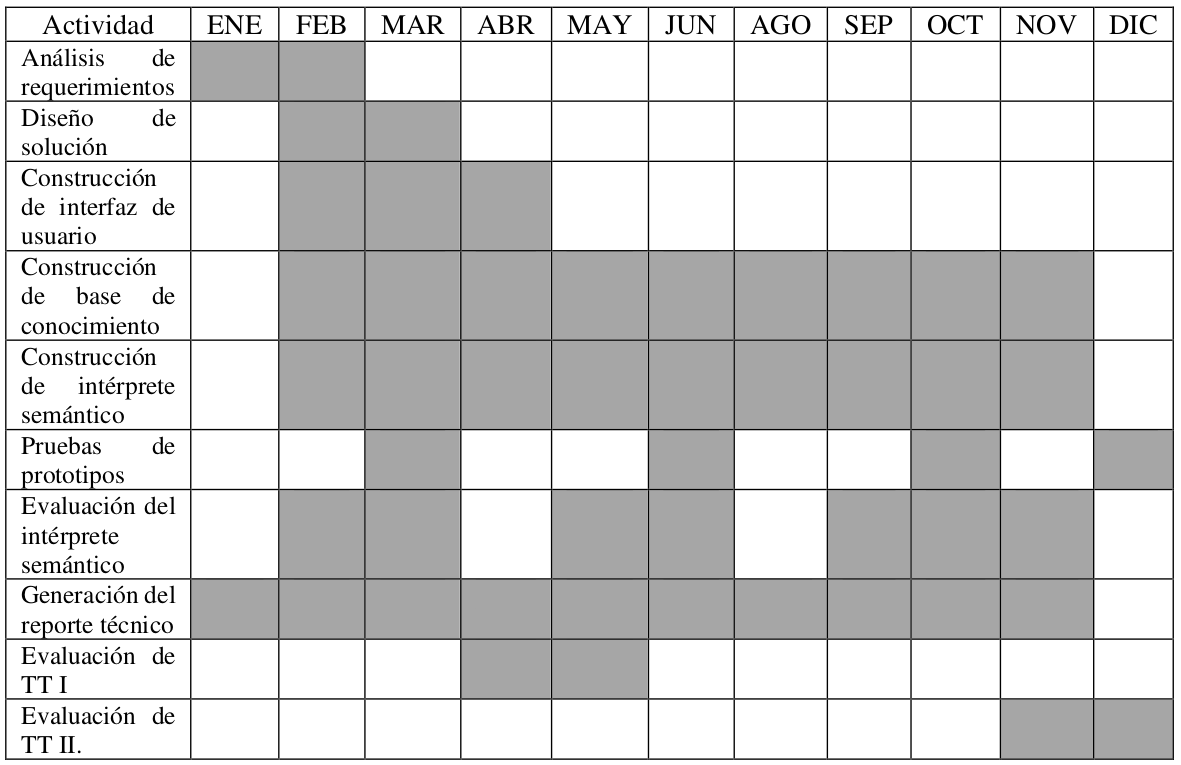
\includegraphics[scale=0.38]{images/4/cronograma}
    \caption{Cronograma de actividades para el desarrollo de este proyecto.}
    \label{fig:cronograma}
\end{figure}

\chapter{Diseño}

En este capítulo se describirá el diseño de esta aplicación para poder llevar acabo este flujo. A muy alto nivel, el flujo de la aplicación es el siguiente:

\begin{enumerate}
    \item El usuario introduce un mensaje.
    \item El cliente envía el mensaje al chatbot.
    \item \label{itm:paso-respuesta} El chatbot recibe el mensaje del usuario e inicia un proceso de formulación de la respuesta basada en la \textbf{intención} y las \textbf{entidades} semánticas del mensaje.
    \item El chatbot envía la respuesta al usuario.
\end{enumerate}

Cabe mencionar que cada mensaje enviado no requiere de un estado ni una sesión, por lo que el diseño de esta aplicación con el flujo descrito asume que \textbf{únicamente el mensaje contiene la información necesaria para poder responderlo.}

\section{Arquitectura de la Aplicación}

El desarrollo de esta aplicación requiere de los siguientes componentes:

\begin{figure}[ht]
    \centering
    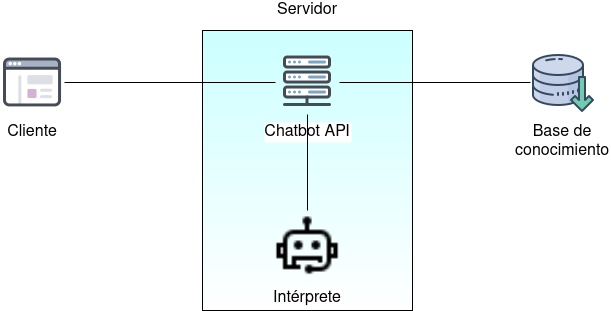
\includegraphics[scale=0.6]{images/5/arquitectura-general.png}
    \caption{Arquitectura de los componentes del sistema.}
    \label{fig:arquitectura-general}
\end{figure}

\begin{itemize}
    \item \textbf{Cliente}: Es la herramienta que solicita los servicios, utilizada por un usuario para poder enviar un mensaje mediante el chat.
    \item \textbf{Chatbot API}: Es la puerta de enlace al API del chatbot. Recibe peticiones HTTP que contienen un mensaje y devuelve una respuesta para el chat del cliente.
    \item \textbf{Intérprete}: Componente de procesamiento de lenguaje natural que procesa la interpretación del mensaje y construcción de las respuestas.
    \item \textbf{Base de Conocimiento}: Base de datos con los documentos normativos y la representación semántica de los mismos utilizada por el Intérprete.
\end{itemize}

\section{Fases del diseño}

Para desarrollar la aplicación, se requiere las siguientes fases de diseño:

\begin{enumerate}
    \item Diseño de la base de conocimiento
    \item Diseño del chatbot
    \item Diseño del sistema cliente
\end{enumerate}


\section{Diseño de la Base de Conocimiento}

En esta fase se pretende modelar el conocimiento y su proceso de estructuración a un formato que el chatbot usará para responder preguntas.

\subsection{Modelo de datos}

\begin{figure}[ht]
    \centering
    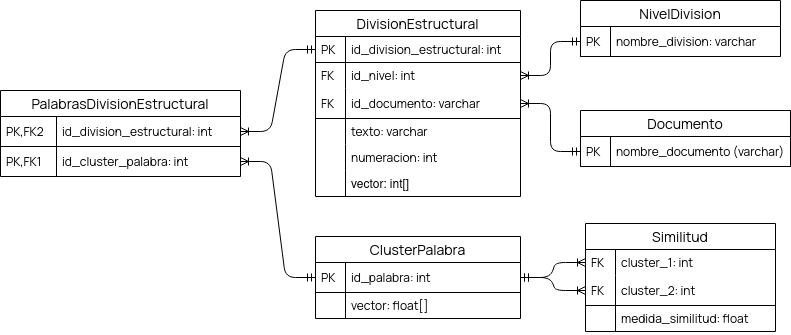
\includegraphics[scale=0.55]{images/5/diagrama-relacional.png}
    \caption{Modelo Relacional.}
    \label{fig:diagrama-relacional}
\end{figure}

Con este modelo se pretende persistir los elementos de los documentos normativos, así como una representación necesaria para que el intérprete pueda procesarlos.

\begin{enumerate}
    \item \textbf{NivelDivision}: Catálogo de los elementos de la división estructural de la ley definidos en el requisito funcional \ref{itm:consultar-reglamento}.
    
    \begin{itemize}
        \item \textbf{nombre\_division}: llave primaria, identifica al nivel en las categorías de \textit{título}, \textit{capítulo}, \textit{sección} o \textit{artículo}.
    \end{itemize}
    
   \item \textbf{Documento}: Son los documentos que contienen los reglamentos del Instituto Politécnico Nacional. Su función es recopilar los reglamentos.
   
   \begin{itemize}
        \item \textbf{nombre\_documento}: llave primaria, nombre que identifica al documento normativo (e.g. \textit{Reglamento Interno del Instituto Politécnico Nacional}).
    \end{itemize}
   
   \item \textbf{DivisionEstructural}: Segmento estructural de los documentos legales. Contienen el texto como tal de los reglamentos:
   
   \begin{itemize}
        \item \textbf{id\_division\_estructural}: llave primaria, es el identificador único del reglamento.
        \item \textbf{id\_nivel}: llave foránea, referencia a la tabla \textbf{Nivel}.
        \item \textbf{id\_documento}: llave foránea, referencia a la tabla \textbf{Documento}.
        \item \textbf{texto}: Contenido textual del reglamento.
        \item \textbf{numeracion}: la enumeración del elemento correspondiente a su nivel (e.g., titulo \textit{1}, artículo \textit{25}, sección \textit{2})
        \item \textbf{vector}: Representación del texto en vector binario que codifica el conocimiento. Su uso se explicó en la sección \ref{sec:deteccion-parafrasis}. 
    \end{itemize}
   
   \item \textbf{PalabraCluster}: Tabla que contiene la representación vectorial de un conjunto de palabras del vocabulario. Su propósito se definió en la sección. \ref{subsec:reduccion-vocabulario}.
   
   
   \begin{itemize}
       \item \textbf{id\_cluster}: llave primaria, identificador del cluster y \textit{también funciona como índice del vector (vector unitario)} para su vector unitario.
       \item \textbf{palabra}: cadena de texto representando a la palabra del vocabulario.
   \end{itemize}
   
   \item \textbf{Similitud}: Tabla representando la similitud entre dos palabras, cuya llave primaria se constituye de las llaves foráneas de ambas palabras:
   
   \begin{itemize}
       \item \textbf{palabra\_1}: llave foránea, referencia a la a tabla \textbf{PalabraCluster}.
       \item \textbf{palabra\_2}: llave foránea, referencia a la a tabla \textbf{PalabraCluster}.
       \item \textbf{medida\_similitud}: similitud cuantificada de acuerdo a un modelo lingüístico utilizando un espacio vectorial entrenado previamente.
   \end{itemize}

    \item \textbf{PalabrasDivisionEstructural}: Relación de muchos a muchos de las tablas \textbf{DivisionEstructural} y \textbf{ClusterPalabra}. Su propósito es agrupar las palabras existentes en el texto para agilizar la construcción del vector binario.
\end{enumerate}

\subsection{Diagrama de Actividad: Transformación y Carga de Documentos Normativos}

\begin{figure}[ht]
    \centering
    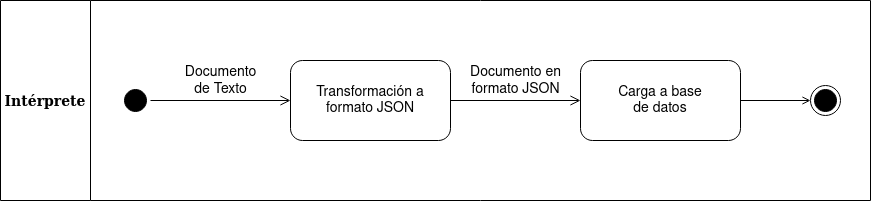
\includegraphics[scale=0.54]{images/5/actividad-transformacion.png}
    \caption{Proceso de transformación y carga de reglamentos estructurados.}
    \label{fig:actividad-transformacion}
\end{figure}

En este proceso, se transforma de manera uniforme a documentos del marco normativo en una estructura útil para el chatbot. Se elige un formato TXT semi-estructurado que separdo por líneas de salto cada título, capítulo, sección y artículo. Este se transforma a un archivo JSON con estructura jerárquica por la naturaleza de los reglamentos. Esto ayuda a revisar también la consistencia del archivo de texto.

\begin{enumerate}
    \item \textbf{Transformación a formato JSON}: Recibe como entrada un archivo semi-estructurado y produce un archivo en formato JSON con la siguiente estructura:
    
    \begin{itemize}
        \item \textbf{items}: arreglo de objetos con los siguientes atributos:
        
        \begin{itemize}
            \item \textbf{contenido}: objeto anidado recursivo
            \item \textbf{enumeracion}: número de elemento de la división estructural
            \item \textbf{texto}: contenido textual del elemento
        \end{itemize}
        
        \item \textbf{nivel}: nombre del nivel de la división estructural
    \end{itemize}
    
    \item \textbf{Carga a base de datos}: Se recibe como entrada el archivo JSON estructurado jerŕquicamente y se recorre en forma de árbol a todos sus elementos para posteriormente cargarlo en la tabla \textbf{DivisionEstructura} del modelo de datos.
\end{enumerate}


%
%
%   DISEÑO DEL CHATBOT
%
%


\section{Diseño del Chatbot}

\subsection{Diseño del Algoritmo de Detección de Paráfrasis}

La medida de similitud de palabras requiere de una representación de word embedding sobre un espacio vectorial, que se obtiene mediante métodos de aprendizaje automático utilizando redes neuronales. Cabe mencionar que \textbf{la construcción del modelo para representar palabras de esta manera está fuera del alcance de este proyecto}.

La consulta introducida será de la siguiente forma:

\begin{itemize}
    \item ¿Cuáles artículos hablan acerca de la \underline{baja temporal del semestre}?
    \item ¿Me puedes decir cuáles reglamentos hablan sobre \underline{rayar o dañar propiedad de la escuela}?
\end{itemize}

El segmento subrayado será nuestra oración de interés y deberá estar sujeto a los requisitos mencionados para la preparación de los datos. Posteriormente, se ejecutará lo siguiente:

\begin{enumerate}
    \item Se quitan las palabras irrelevantes o vacías(stop words) de la consulta y las resultantes se llevarán a su forma lematizada.
    \item Se construye el vector de consulta $q$: se establece un valor de 1 en todos los índices del vector cuya dimensión pertenece a una palabra presente en la consulta, de lo contrario se establece en 0 (i.e., es la suma de los vectores unitarios de las palabras que aparecen en la consulta.)
    \item Se iterarán sobre todos los artículos $a$ de un reglamento y se ejecutará la función de similitud entre el vector de consulta mediante $sim(q, a)$.
    \item Se ordenarán conforme al resultado de relevancia obtenido por la función de similitud y se obtendrán todos aquellos que superen un umbral $sim(q, a)  > 0.7$.
    \item Se devuelve como salida del algoritmo la lista de artículos que cumplen la condición anterior.
\end{enumerate}

\begin{figure}
    \begin{algorithm}[H]
        \SetAlgoLined
        \SetKwInput{Entrada}{Entrada}
        \SetKwInput{Salida}{Salida}
        \SetKwFor{ParaCada}{ParaCada}{hacer}{fin para cada}
        \SetKwIF{SSi}{EnOtroCasoSi}{EnOtroCaso}{si}{entonces}{sin ́o, si}{sin ́o}{fin si}

        \Entrada{Cadena de texto $q$ con la consulta del usuario.}
        \Salida{Lista de artículos $a$ relevantes a la consulta.}
        
        $q_{norm}$ = quitar\_palabras\_vacias($q_entrada$)\;
        $q_w$ = lematizar($q_{norm}$)\;
        $q_v$ = vectorizar($q_w$)
        umbral\_aceptable\_similitud = 0.7\;
        articulos\_relevantes = inicializar\_lista\_vacia()\;
        \ParaCada{articulo  $a$ en la base de conocimiento}{
            $a_v$ = vectorizar($a$)\;
            nivel\_parafrasis = calcular\_similitud($q_v$, $a_v$)\;
            \SSi{nivel\_parafrasis $\geq$ umbral\_aceptable\_similitud}{
                agregar(articulos\_relevantes, $a$)\;
            }
        }
        \caption{Algoritmo de detección de paráfrasis.}
    \end{algorithm}
    \label{fig:algoritmo-deteccion-parafrasis}
\end{figure}

\newpage

\subsection{Diagrama de Secuencia: Interacción Usuario-Chatbot}

En la figura \ref{fig:secuencia-general} se muestra el diagrama de secuencia, el cual contiene un bloque denominado \textbf{Formular respuesta}. Este bloque se ejecutará de acuerdo a las intenciones detectadas y que se describieron en en el requisito funcional \ref{itm:requisito-intenciones}.


Cabe mencionar que la intención \textit{Buscar conceptos} es el que ejecutará el algoritmo descrito en la figura \ref{fig:algoritmo-deteccion-parafrasis}.

\begin{figure}[ht]
    \centering
    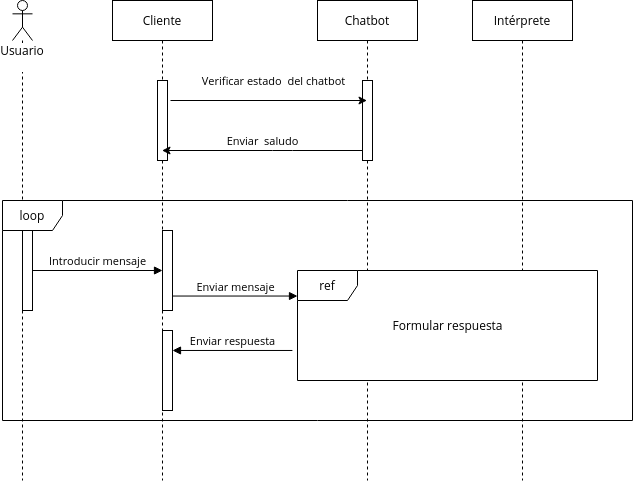
\includegraphics[scale=0.7]{images/5/diagrama-secuencia.png}
    \caption{Diagrama de la secuencia Interacción Usuario-Chatbot.}
    \label{fig:secuencia-general}
\end{figure}

\newpage

\subsection{Diagrama de Actividad: Reducir Vocabulario}
\label{subsec:reduccion-vocabulario}

El español tiene 88,000 palabras en su diccionario. Cargar en memoria todas las palabras y calcular una matriz de similitud $M_{88000,88000}$ requiere de 7,744,000,000 operaciones con sus respectivas asignaciones de memoria, que podría requerir hasta 1 TB de memoria.

Es por esto que se buscará reducir los vectores de palabras reduciéndolos a \textbf{clusters} de palabras, que realmente es reducir un grupo de vectores al promediarlos dando por resultado un centro de esa agrupación que se vuelve el nuevo vector de palabra.

La agrupación de estos vectores de palabras son \textit{semánticamente similares}, por lo que deberían significar lo mismo o algo parecido. Entonces se buscará reducir la cantidad de vectores para optimizar procesamiento y almacenamiento, pero la cantidad reducida no debe afectar \textit{la distribución de vectores para no perder su valor semántico}.

\begin{figure}[ht]
    \centering
    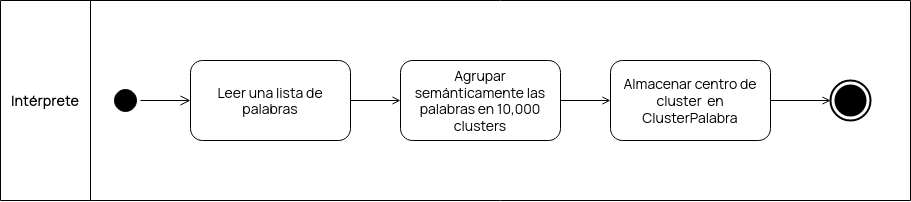
\includegraphics[scale=0.5]{images/5/actividad-reducir-vocabulario}
    \caption{Diagrama de la actividad: Reducir vocabulario.}
    \label{fig:reducir-vocabulario}
\end{figure}

La figura \ref{fig:reducir-vocabulario} describe el proceso a un nivel general. En esta actividad se detalla la reducción del vocabulario, promediando las representaciones vectoriales en agrupaciones utilizando el algoritmo K-Means.

\begin{enumerate}
    \item \textbf{Leer lista de palabras}: Se lee un archivo de texto con el vocabulario de entrenamiento con palabras en español.
    \item \textbf{Agrupar semánticamente las palabras en 10,000 clusters}: Se agrupan las palabras en 10,000 clusters utilizando la similitud de palabras cono medida de distancia.
    \item \textbf{Almacenar centro de cluster en ClusterPalabra}: El resultado de las agrupaciones se almacenan en la tabla \textbf{ClusterPalabra}.
\end{enumerate}

\subsection{Diagrama de Actividad: Inicialización}

\begin{figure}[ht]
    \centering
    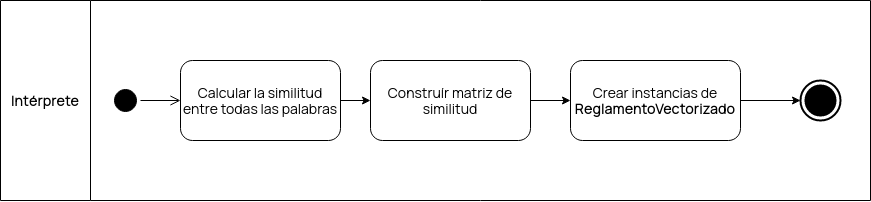
\includegraphics[scale=0.5]{images/5/actividad-inicializacion}
    \caption{Diagrama de la actividad: Inicialización de matriz de similitud y vector de palabras.}
    \label{fig:actividad-inicializacion}
\end{figure}

Antes de que el servicio del chatbot se encuentre funcional, la primera actividad que debe ejecutarse es la de inicialización del modelo utilizado en el algoritmo \ref{fig:algoritmo-deteccion-parafrasis} (la matriz $\mathbf{W}$). La similitud calculada se almacena en la tabla \textbf{Similitud} de la figura \ref{fig:diagrama-relacional} para posteriormente poblar la matriz.

Los pasos de esta actividad son:

\begin{enumerate}
    \item \textbf{Calcular la similitud entre todas las palabras}: Utilizando un modelo de espacio vectorial, iterar sobre todos las instancias de \textbf{ClusterPalabra} y calcular su similitud con todos las otras instancias de \textbf{ClusterPalabra}, incluso consigo mismo.
    \item \textbf{Construir matriz de Similitud}: Los elementos de la matriz se llenarán como se especifica en la sección \ref{fig:algoritmo-deteccion-parafrasis}; es decir, el índice del renglón y la columna será \textbf{id\_palabra} por lo que la dimensión de los vectores y la cantidad de columnas y renglones de $\mathbf{W}$ son la cantidad de instancias en \textbf{ClusterPalabra}.
    \item \textbf{Poblar tabla ReglamentoVectorizado}: Representar cada elemento de la tabla \textbf{DivisiónEstructural} que sea artículo en su representación binaria; por cada palabra que aparezca en su texto, obtener su \textbf{ClusterPalabra} a la que pertenece y establecer un valor de 1 en el índice indicado por el identificador de \textbf{ClusterPalabra}.
\end{enumerate}



\subsection{Diagrama de Actividad: Formular respuesta}
\label{subsec:formular-respuesta}

Esta actividad es el detalle de lo que ocurre cuando se requiere atender un mensaje de un usuario, especificado en el diagrama de secuencia del proceso general de la aplicación en la figura \ref{itm:requisito-intenciones}. El proceso se desribe de la siguiente manera:

\begin{enumerate}
    \item \textbf{Recibe mensaje}: Se recibe la cadena de texto que introduce el usuario a través del cliente.
    \item \textbf{Reconocer intención}: La cadena de texto se introduce a un clasificador de intenciónes que categoriza la intención en una de las siguientes: {\textit{saludar}, \textit{despedir}, \textit{solicitar\_reglamento}, \textit{buscar\_conceptos}}.
    \item \textbf{Se evalúa la intención y se elige una acción}
    
    \begin{enumerate}
        \item La intención es \textit{saludar}: Se elige un mensaje del catálogo de saludos de acuerdo a la hora del día y se informa acerca del uso de la aplicación (i.e., que cosas puede hacer y ejemplos de mensajes).
        \item La intención es \textit{despedir}: Se elige un mensaje del catálogo de despedidas.
        \item La intención es \textit{solicitar\_reglamento}: 
        
        \begin{enumerate}
            \item \textbf{Extraer entidades: nivel de reglamento y número}: Del mensaje del usuario se reconoce y se extraen la entidades \textbf{nivel}, que representa el nivel de división estructural, y \textbf{número} que representa la enumeración en el documento normativo.
            \item \textbf{Recuperar reglamento}: utilizando el \textbf{nivel} y \textbf{enumeración}
        \end{enumerate}
        
        \item La intención es \textit{buscar\_conceptos}: Se ejecuta lo siguiente
        
        \begin{enumerate}
            \item \textbf{Extraer enunciado}: se elimina la parte solicitante (\textit{qué artículos hablan acerca de..., en dónde dice que...}) del mensaje y se regresa única mente el texto con los conceptos relevantes, el cual es básicamente el restod e la oración
            \item \textbf{Ejecutar algoritmo de similitud de conceptos sobre todos los artículos}: Iterar sobre todos los elementos de \textbf{ReglamentoVectorizado} y regresar una lista de todos los \textbf{artículos} vector tenga una similitud por encima del 0.5.
            \item \textbf{Recuperar artículos}: Recuperar cada \textbf{artículo} de los documentos normativos y regresar un mensaje con la lista de artículos recuperados.
        \end{enumerate}
        
        \item La intención es \textit{desconocida}: Se regresa un mensaje al usuario indicando que no se reconoce lo que quiere hacer, agregando información acerca de lo que el chatbot puede hacer.
    \end{enumerate}
    
    \item La intención es \textit{desconocida}: Esto ocurre cuando no se entiende lo que el usuario quiere. Se regresa un mensaje informativo al usuario indicando de las funciones que hace el chatbot.
    
    \item \textbf{Devolver respuesta}: El mensaje construido se devuelve al cliente que solicitó el servicio del chatbot.
\end{enumerate}

\newpage

\begin{figure}[ht]
    \centering
    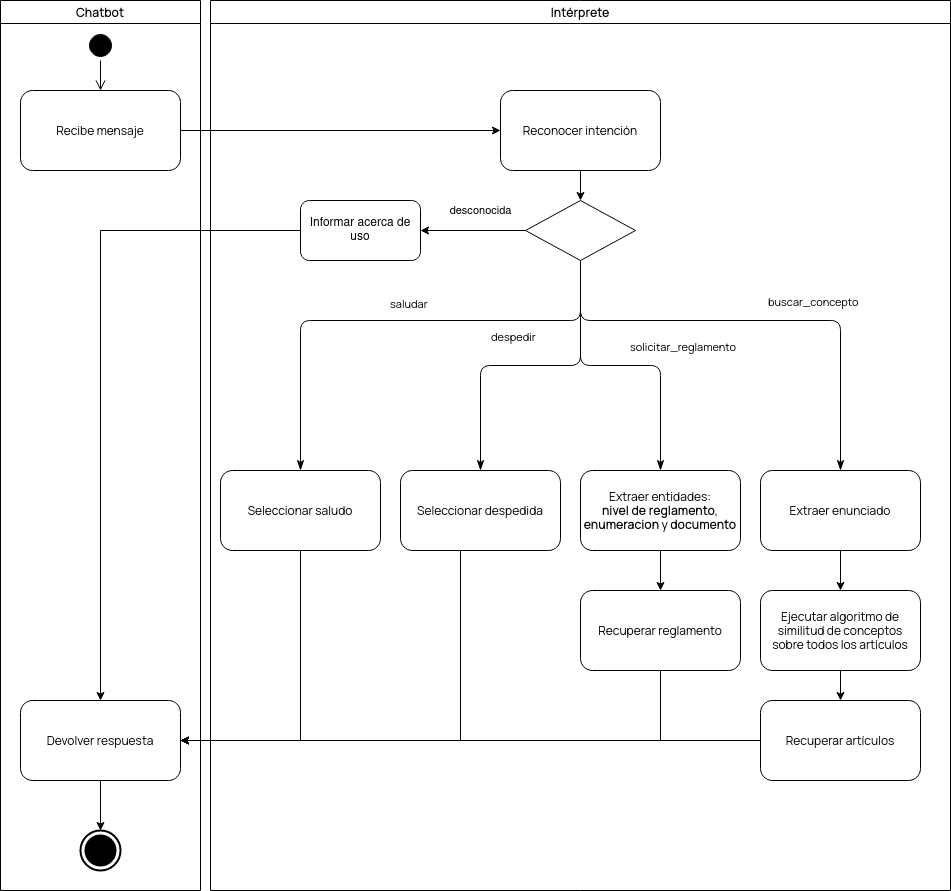
\includegraphics[scale=0.49]{images/5/diagrama-actividades}
    \caption{Diagrama de la actividad: Formular Respuesta.}
    \label{fig:actividad-responder}
\end{figure}


%
%
%   DISEÑO DE LA INTERFAZ DE USUARIO
%
%

\newpage

\section{Diseño del Sistema Cliente}

\subsection{Casos de Uso}

\begin{figure}[ht]
    \centering
    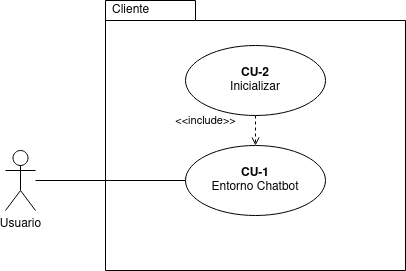
\includegraphics[scale=0.61]{images/5/casos-de-uso}
    \caption{Representación del caso de uso del usuario mediante el cliente.}
    \label{fig:diagrama-casos-de-uso} 
\end{figure}

\subsubsection{Actores}

Debido a que este sistema proporciona un chatbot disponible para el público de la comunidad de ESCOM, se define solo un actor que realiza una interacción con el sistema:

\begin{itemize}
    \item \textbf{Usuario}: Es todo aquel que usa el sistema que usa el sistema como herramienta auxiliar para la asesoría. Obtiene su utilidad al utilizar el sistema cliente enviando mensajes de texto al chatbot.
\end{itemize}

\subsection{Descripción de los casos de uso}
\label{sec:casos-de-uso}

% Listado de casos de uso
\noindent\makebox[\linewidth]{\rule{\textwidth}{0.4pt}}
\begin{enumerate}[leftmargin=2.5cm ,label={\bfseries CU-\arabic*}]
    
    % Inicia CU
    \item \textbf{Entorno Chatbot}: 
    
        \textbf{Descripción}: Permite la interacción entre el usuario y el chatbot para enviar mensaje.
        
        \textbf{Pre-condiciones}: 
        
        \begin{itemize}
            \item Debe haber una conexión con el servidor
        \end{itemize}
        
        \textbf{Post-condiciones}: 
        
        \begin{itemize}
            \item No existe post-condición.
        \end{itemize}
        
        \textbf{Errores}: 
        
        \begin{itemize}
            \item No se puede acceder al servidor.
        \end{itemize}
        
        \textbf{Flujo}:
        
        \begin{enumerate}[label=\arabic*)]
            \item El Usuario escribe mensaje.
            \item El Usuario envía mensaje al servidor.
            \item El Usuario espera respuesta del chatbot.
            \item Trayectoria alternativa A:

                \begin{itemize}
                    \item El cliente recibe respuesta del chatbot.
                    \item El cliente muestra el mensaje de respuesta al mensaje del usuario.
                \end{itemize}

            \item Trayectoria alternativa B:

                \begin{itemize}
                    \item El cliente no puede acceder al servidor.
                    \item El cliente muestra un mensaje en el \textbf{Área de Diálogo} diciendo: "No se pudo conectar con el chatbot. Intente de nuevo mas tarde."
                \end{itemize}
            \item Continúa en paso 1.
        \end{enumerate}
        \noindent\makebox[\linewidth]{\rule{\textwidth}{0.4pt}}
    
    % Inicia CU
    \item \textbf{Inicializar}: 
    
        \textbf{Descripción}: El entorno del chat revisa el estado del servicio web del Chatbot y actualiza el entorno.
        
        \textbf{Pre-condiciones}: 
        
        \begin{itemize}
            \item El usuario se encuentra en el sitio de la aplicación.
            \item La interfaz de usuario se ha cargado.
        \end{itemize}
        
        \textbf{Post-condiciones}: 
        
        \begin{itemize}
            \item Se muestra un mensaje de saludo del chatbot.
        \end{itemize}
        
        \textbf{Errores}: 
        
        \begin{itemize}
            \item El cliente no logra realizar una petición al chatbot.
            \item El chatbot responde con un mensaje que indica que el servicio no esta disponible.
        \end{itemize}
        
        \textbf{Flujo}:
        
        \begin{enumerate}[label=\arabic*)]
            \item El cliente del entorno del chat manda una peticion HTTP al chatbot.
            \item El cliente se queda a la espera de la respuesta del chatbot.
            \item El cliente recibe una respuesta HTTP del chatbot.
            \item Trayectoria alternativa A:
                \begin{enumerate}[label=\arabic*)]
                    \item El mensaje que recibe el el entorno chat tiene un estado 200:
                    \item Se extrae el \textit{saludo} del chatbot incluido en la respuesta.
                    \item Se renderiza el mensaje en el \textbf{Area de dialogo}, colocando el mensaje en la esquina superior izquierda.
                \end{enumerate}

            \item Trayectoria alternativa B:
                \begin{enumerate}[label=\arabic*)]
                    \item El mensaje tiene un estado diferente a 200:
                    \item Se renderiza un mensaje en el \textbf{Área de dialogo}, con el texto \textit{"Servicio no disponible por el momento. Intente de nuevo mas tarde."}, colocando el mensaje en la esquina superior izquierda.
                \end{enumerate}
            \item Fin de caso de uso.
        \end{enumerate}
\end{enumerate}
\noindent\makebox[\linewidth]{\rule{\textwidth}{0.4pt}}

\newpage

\subsection{Diseño de la Interfaz de Usuario}

\subsubsection{UI-Entorno-Chat}
\label{subsubsec:ui-entorno-chat}

El entorno del chat se constituye de 3 elementos:

\begin{itemize}
    \item \textbf{Área de diálogo}: Es la parte en la que aparecen los mensajes en forma de burbuja conversacional. Los mensajes del chatbot estarán del lado izquierdo mientras que los del usuario del lado derecho.
    \item \textbf{Área de entrada de texto}: Es el lugar en donde el Usuario introduce el texto a mandar como mensaje al chatbot.
    \item \textbf{Botón de envío}: Su función es la de enviar el mensaje introducido en el \textbf{área de entrada de texto} y limpiarlo una vez obtenido.
\end{itemize}

\begin{figure}[ht]
    \centering
    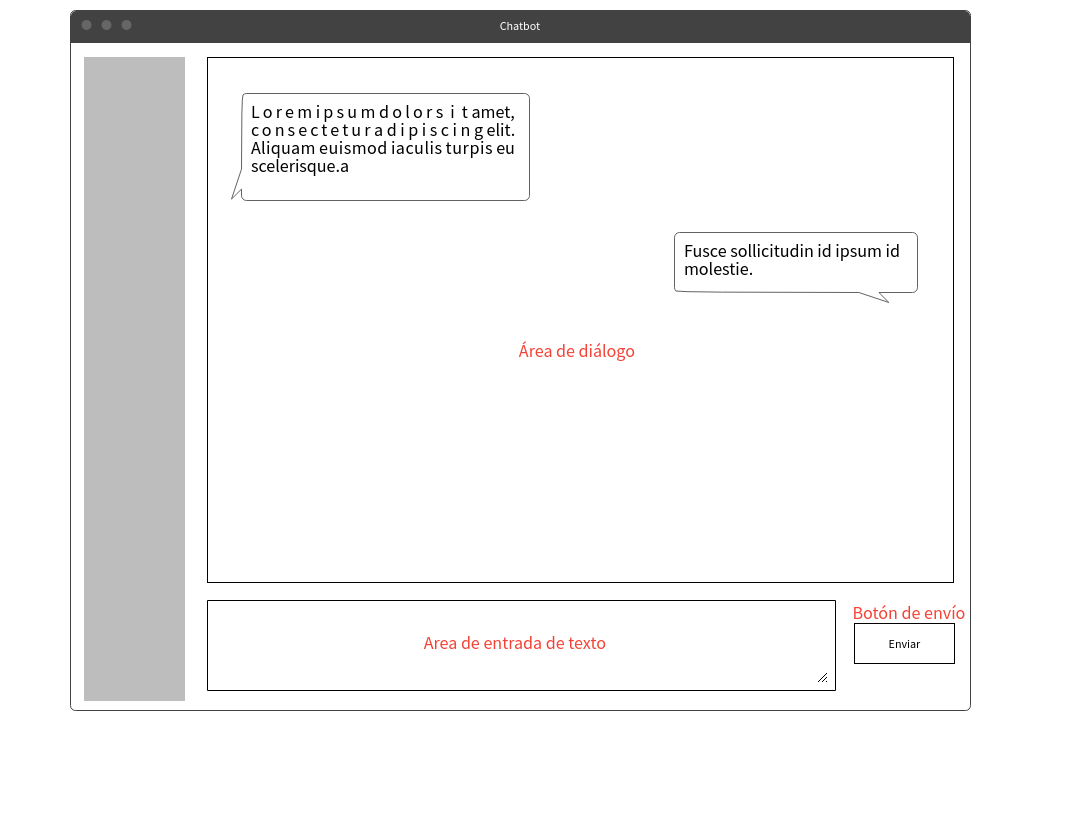
\includegraphics[scale=0.425]{images/5/interfaz-usuario}
    \caption{Diseño de la ventana de la interfaz de usuario mediante un navegador web.}
    \label{fig:interfaz-usuario}
\end{figure}

\chapter{Desarrollo}

\section{Primera Iteración}

\subsection{Extracción de Texto de los Documentos del Marco Normativo}

Como se mencionó en la sección \ref{subsec:marco-normativo-ipn}, el IPN ofrece accesibilidad al conjunto de documentos que conforman el marco normativo. Existe un problema en utilizar estos documentos como fuente de información para el sistema propuesto en este trabajo terminal: \textbf{la divulgación de estos documentos se hacen en formato PDF}. Los formatos PDF agregan un formato de organización gráfica iy visual, pero no son óptimos para procesos de extracción.


\begin{figure}[ht]
    \centering
    \fbox{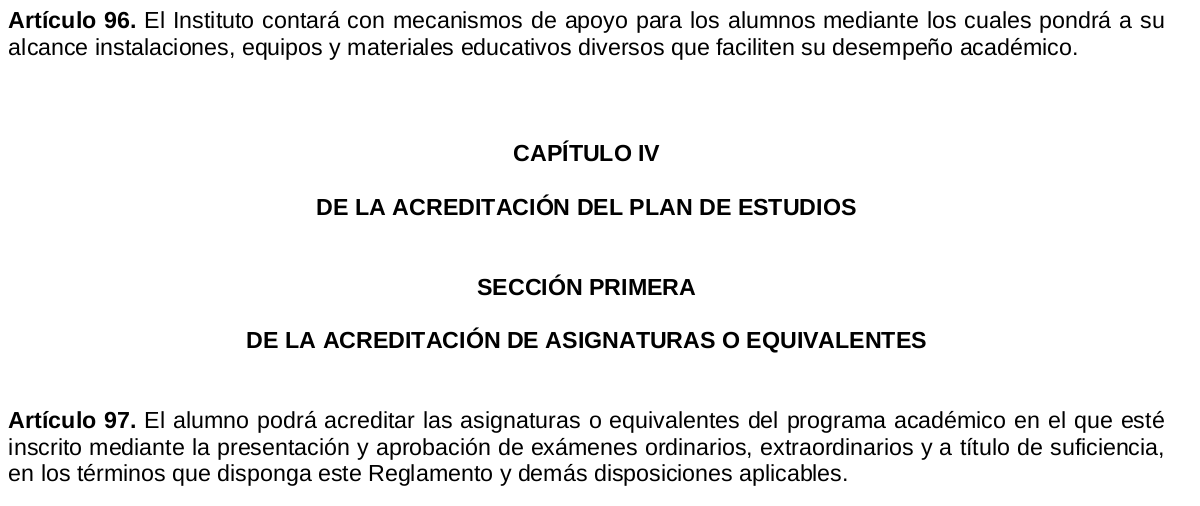
\includegraphics[scale=0.38]{6/ejemplo_reglamento_1}}
    \caption{Segmento del Reglamento Interno del Instituto Politécnico Nacional}
    \label{fig:ejemplo_1_reglamento_interno}
\end{figure}

\begin{figure}[ht]
    \centering
    \fbox{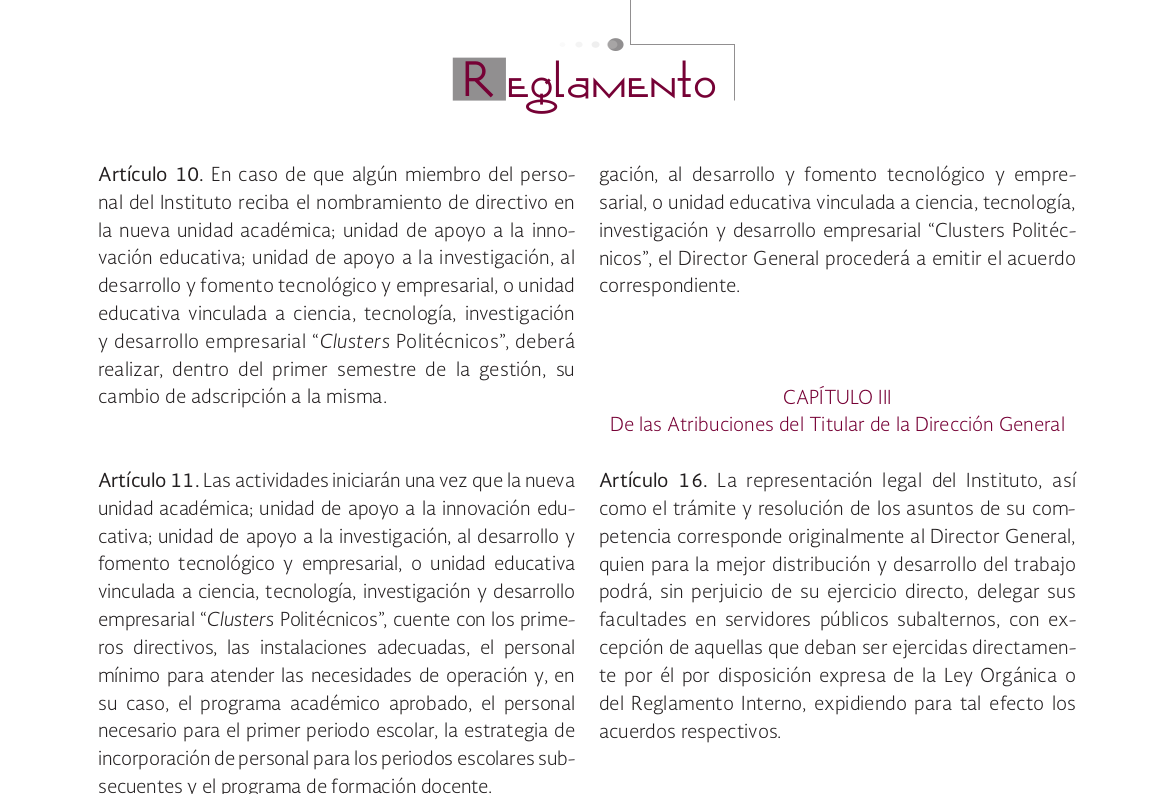
\includegraphics[scale=0.39]{6/ejemplo_reglamento_2}}
    \caption{Segmento del Reglamento Orgánico del Instituto Politécnico Nacional}
    \label{fig:ejemplo_2_reglamento_organico}
\end{figure}

\begin{figure}[ht]
    \centering
    \fbox{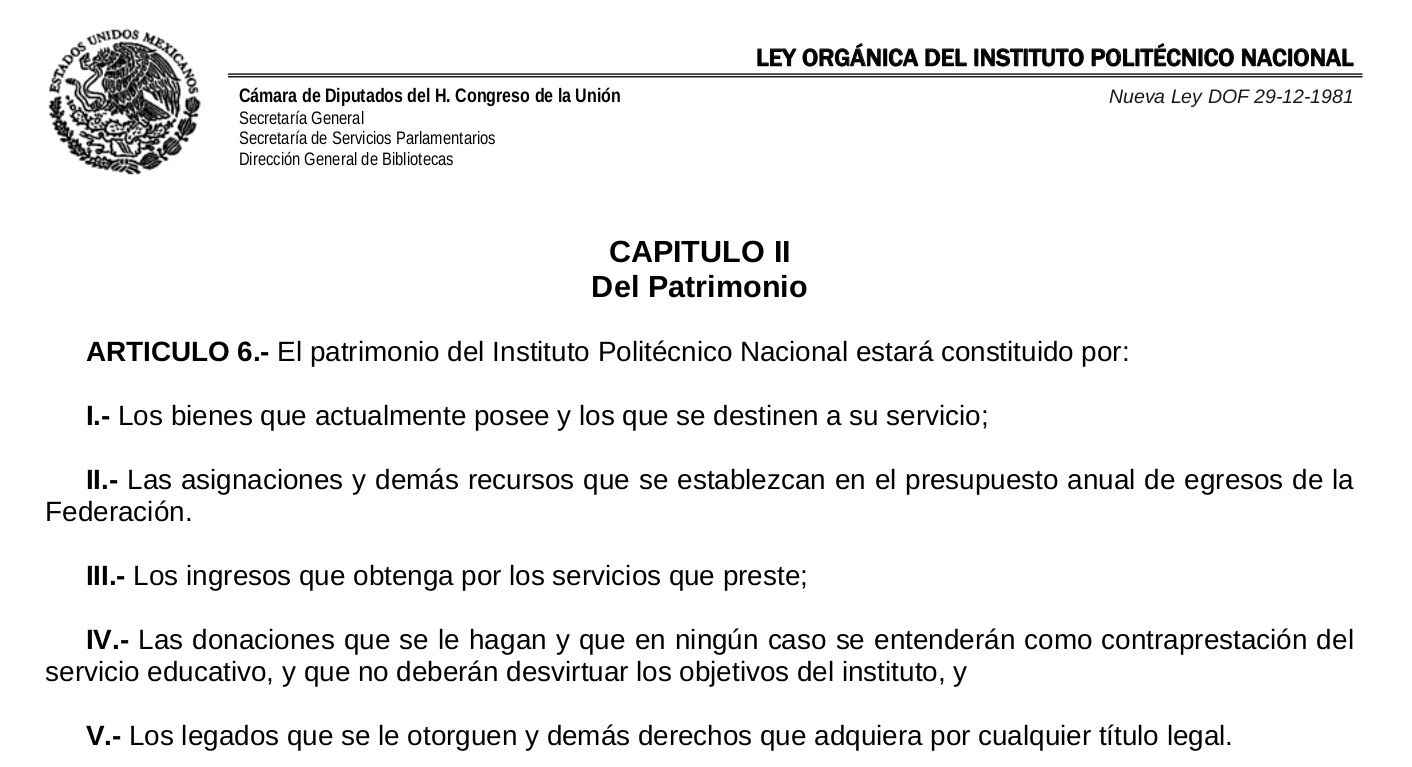
\includegraphics[scale=0.32]{6/ejemplo_reglamento_3}}
    \caption{Segmento de la Ley Orgánica del Instituto Politécnico Nacional}
    \label{fig:ejemplo_3_ley_organica}
\end{figure}

El problema general es este: la figura \ref{fig:ejemplo_1_reglamento_interno} muestra una manera muy sencilla de organización textual de la información, pero difiere mucho en cuanto a la organización de contenido de la figura \ref{fig:ejemplo_2_reglamento_organico}. Mas aún, la figura \ref{fig:ejemplo_3_ley_organica} añade a la estructura de la página una cabecera con nombres de una institución y sus direcciones internas, las cuáles son irrelevantes en cuanto al contenido normativo de nuestro interés.
 
Por lo tanto, podemos concluir que un estándar de división estructural normativa no es suficiente en sí, sino también \textbf{se debe estandarizar la forma en cómo se representan esos datos cuando se almacenan}. Esto es un problema de \textbf{serialización} de datos en la que no existe un formato unificado semántico. Se debe extraer esta información para posteriormente unificar su formato. Esto es el siguiente paso de la preparación del texto.

A pesar de que son relativamente pocos documentos, la cantidad de texto contenido dentro de ellos es grande como para extraer de manera manual. Sin embargo, para este trabajo terminal se ha decidido \textbf{extraer el texto a mano}. Este método es muy inconveniente por diversas razones. La principal razón que se considera en el desarrollo de este trabajo terminal es por el esfuerzo manual requerido, el cuál hace que el proceso sea propenso a errores. Como consecuencia esto también la cantidad de tiempo invertida en desarrollar este trabajo terminal.

Sin embargo, si se depende de una herramienta que extraiga texto automática mente, resulta en incongruencias como el siguiente segmento de texto extraído de la figura \ref{fig:ejemplo_2_reglamento_organico}:

\begin{quote}
    \textbf{Artículo 10.} En caso de que algún miembro del person-gación, al desarrollo y fomento tecnoloógico y empre-nal del Instituto reciba el nombramiento de directivo en sarial, o unidad educativa vinculada a ciencia, tecnología...
\end{quote}

Esto es debido a que la organización de texto no es la misma que la organización visual de un documento PDF. En este caso, la herramienta de extracción de PDF lo hizo por cada renglón de la página, sin importar que el documento estuviera dividido en dos columnas.

\newpage
\subsubsection{Formato de Documento Normativo de Entrada}

Entonces necesitamos que el documento venga en formato TXT, y que cada \textbf{título}, \textbf{sección}, \textbf{capítulo} y \textbf{artículo} venga separado por dos saltos de línea (\textbackslash n\textbackslash n). Tambien el texto y el nivel estructural debe ser separado con un guin (-) o un punto (.).

\begin{quote}
    \textbf{Capítulo Primero} - Disposiciones Generales
    
    \textbf{Artículo 1}. Las disposiciones del presente Reglamento son de observancia general y obligatoria en el Instituto Politécnico Nacional.
    
    \textbf{Artículo 2}. Este ordenamiento tiene por objeto establecer las condiciones que regulan el ingreso, la trayectoria escolar, la permanencia y el egreso de alumnos que cursen algún programa académico de los niveles medio superior, superior y posgrado, así como de los usuarios de todos aquellos programas que se ofrezcan para complementar su formación y con fines de capacitación, actualización técnica y profesional, formación empresarial, educación continua, y enseñanza de lenguas extranjeras en las unidades académicas, unidades de apoyo a la innovación educativa, unidades de apoyo a la investigación y al fomento y desarrollo empresarial y demás áreas referidas en el artículo 2 del Reglamento Orgánico, en las modalidades educativas que ofrece el Instituto Politécnico Nacional.
    
    \textbf{Artículo 3}. Para efectos del presente Reglamento se entenderá por:
    Academia: Al órgano constituido por profesores que tiene la finalidad de proponer, analizar, opinar, estructurar y evaluar el proceso educativo.
    ...
\end{quote}

Por ejemplo:

\begin{itemize}
    \item El primer elemento sería el capítulo primero, se separa el texto de su nivel mediante el guión. Posteriormente se introducen dos saltos de línea para separarlo del artículo 2. 
    \item El tercer elemento es el artículo 3. Este tiene mas de un párrafo, por lo que un solo salto de línea separa sus párrafos pero no lo separa del artículo siguiente hasta que encuentre los dos saltos de línea.
\end{itemize}

Los documentos normativos extraidos manualmente a un formato TXT se pueden encontrar en el siguiente repositorio: \url{https://github.com/AranGarcia/Shepard}.

\subsubsection{Estructura Propuesta}

Una vez obtenido el formato TXT de entrada, se utilizará como entrada al sistema para su almacenamiento en la base de conocimiento.

Para estructurar los reglamentos, se toma en cuenta la jerarquía de su división estructural mientras se mantenga el contenido textual así como la enumeeración. Es por eso que se propone la siguiente estructura:

\begin{itemize}
    \item \textbf{items}: arreglo de objetos con los siguientes atributos:
    
    \begin{itemize}
        \item \textbf{contenido}: objeto anidado recursivo
        
        \begin{itemize}
            \item \textbf{items}: ...
            \item \textbf{nivel}: ...
        \end{itemize}
        
        \item \textbf{enumeracion}: número de elemento de la división estructural
        \item \textbf{texto}: contenido textual del elemento
    \end{itemize}
    
    \item \textbf{nivel}: nombre del nivel de la división estructural
\end{itemize}

Este formato es para mantener una forma jerárquica inherente en los documentos normativos discutidos anteriormente y que se les denomina divisón estructural. Entonces se desarrollará un programa que dado un documento normativo TXT lo transforme a la estructura propuesta.

\begin{figure}
    \centering
    \lstinputlisting[language=yaml]{src/3/ejemplo-estructura.yaml}
    \caption{Estructura propuesta inicialmente para organizar texto mediante el lenguaje YAML.}
    \label{fig:estructura_propuesta}
\end{figure}

El programa que realiza esto se puede encontrar en el repositorio \url{https://github.com/AranGarcia/Cookie/tree/master/yamlizer}.
\chapter{Experimentación y Pruebas}

Lorem ipsum.
\chapter{Conclusión}

En este proyecto se logró un avance principal en el diseño principal de la estructura de cómo sería una consulta automatizada y qué tecnologías requiere para tal fin. Es suficiente decir que la base de conocimiento fue diseñada para persistir la información necesaria para consultas a los documentos normativos.

Sin embargo, cabe mencionar las dificultades encontradas en la estructuración del conocimiento. Mientras no existan formas estandarizadas de divulgar información semánticamente en los medios digitales, como lo es mediante internet, estos problemas seguirán existiendo. Esto debido a que, hasta la fecha, todavía se dependen de intervención humana para procesos que involucren comunicación o divulgación de información. Se espera que con este proyecto se enfatice la necesidad de estandarizar conocimiento para que una transformación digital de los procesos se hagan de manera óptima para las actividades que hacemos cotidianamente.

En cuanto a los objetivos, se considera que llevaban un avance acorde a lo planeado hasta la primera quincena de marzo. Pero hay que detallar el desvío de atención provocado por una subestimación en la planeación de la construcción de la base de conocimiento. Como se mencionó anteriormente, tenía que estructurarse adecuadamente para utilizarse en este proyecto. Se tuvo que recurrir al proceso manual de extracción a un formato intermedio. Aún así, se considera que las bases de diseño y funcionalidad de este proyecto están firmemente establecidas para que se continúe con las actividades del cronograma hasta concluir con una versión desplegable.


\printbibliography

\end{document}
